% doc type
\documentclass[12pt]{article}

% set up supplemental section
\newcommand{\beginsupplement}{%
	\setcounter{table}{0}
	\renewcommand{\thetable}{S\arabic{table}}%
	\setcounter{figure}{0}
	\renewcommand{\thefigure}{S\arabic{figure}}%
}

% format page, paragraph
\usepackage[margin=1in]{geometry}
\usepackage{lineno}
\linenumbers
\usepackage{setspace}
\doublespacing
\usepackage[utf8]{inputenc}
\usepackage[hidelinks]{hyperref}
\usepackage{authblk}

% bib - uses better biblatex
\usepackage[style=apa,backend=biber]{biblatex}
\addbibresource{./Zotero_adr_dwi.bib}

% figures and tables
\usepackage{graphicx}
\graphicspath{ {./} }
\usepackage{multirow}
\usepackage[table,xcdraw]{xcolor}
\usepackage{url}
\usepackage{float}
\usepackage{longtable}
\usepackage{rotating}

% code
\usepackage{listings,lstautogobble}
\lstset{language=R,
	basicstyle=\small\ttfamily,
	otherkeywords={0,1,2,3,4,5,6,7,8,9},
	morekeywords={TRUE,FALSE},
	deletekeywords={data,frame,length,as,character},
	autogobble=true
}
\renewcommand\lstlistingname{R Code}

% math
\usepackage{amsmath}
\usepackage{caption}
\DeclareCaptionType{equ}[R Code][]

% title page info
\title{Longitudinal study of concussion-related diffusion MRI changes in college athletes}
\date{}

\author[1,*]{Nathan M. Muncy}
\author[1]{Heather C. Bouchard}
\author[1]{Aron K. Barbey}

\affil[1]{Center for Brain, Behavior and Biology, University of Nebraska-Lincoln, Lincoln, Nebraska, USA}
\affil[*]{Corresponding author.	Email: nmuncy2@unl.edu}

% start document
\begin{document}

% title page
\maketitle
\pagebreak


% abstract page
\begin{abstract}

% TODO: Update, finalize.

Sports-related traumatic brain injuries affect 1.6-3.8 million individuals in the US each year, and diffusion weighted imaging can measure the complex timeline of resulting axolemmal changes. Such longitudinal data is difficult to model statistically, however, given the high-dimensionality, semi-parametric and interdependent scalar values, and non-linear spatial (within-tract) and temporal (across visit) properties. Proposal: hierarchical generalized additive models (HGAMs) are well-suited to fit such data with the requisite flexibility and sensitivity to investigate (a) the spatial and temporal changes of white matter tracts, and (b) how such changes relate to diagnostic assessments. Methods: we utilized MRI and IMPACT data collected from 67 college athletes (9 female, age=19.43[1.68]) at three visits: start-of-season, post-concussion, and return-to-play. Diffusion tensors were modeled via constrained spherical deconvolution and probabilistic tractography from pyAFQ yielded 100 scalar values per white matter bundle. Results: By fitting the scalar profiles with longitudinal HGAMs we detected within-tract changes as a function of visit, revealing distinct patterns of post-injury disruption and recovery. Critically, it is unlikely that such changes would have been detected with standard techniques given their linear assumptions and limited dimensionality. Further, we examined whether these evolving diffusion metrics correlated with cognitive outcomes using HGAM tensor product interaction smooths and found moderate evidence linking white matter alterations to IMPACT composite scores. Merit: HGAMs offer a powerful framework to capture the complex progression of brain injury. Our findings suggest that HGAMs enhance our understanding of the spatiotemporal dynamics of brain injury and may enable more accurate tracking of injury and recovery.

\end{abstract}

\vfill
KEYWORDS: DWI, MRI, GAM, TBI, Concussion\\
\pagebreak


\section{Introduction}
\label{sec:intro}

% TODO: (Heather?) Epidemilogic description of TBI in US, athletes
Traumatic brain injury affects [XXX] individuals each year with approximately [XXX] results from sport-related activities, a number which may be under-reported. [TBD - Heather]

% mTBI sequelae description
As rapid acceleration and deceleration of the head results in consequential forces for sensitive neural structures, concussion (e.g. mild traumatic brain injury (mTBI), see \textcite{mayer2017SpectrumMildTraumatic} and \textcite{silverberg2023AmericanCongressRehabilitation}) can result in traumatic axonal injury. Biomechanical insult increases axolemmal permeability to Ca$^{2+}$ which in turn activates proteolytic calpains with consequences for receptors and ionic channels. Structurally, initial stretch and/or secondary calpain-mediated mechanisms can trigger the depolymerization of microtubules (and also the hydrolysis of tubulin and microtubule-associated proteins) resulting in impaired axonal transport. Continued transportation results in the accumulation of axonal transport products (e.g. amyloid precursor protein, APP) appearing as varicosities, with peak APP accumulation occurring around 24 hours post injury. With more severe injuries, significant axolemmal mechanoporation, axonal undulations, and neurofilament pathology can result in substantial cytotoxic edema and even axotomy. In each of these sequelae, the typical diffusion trajectories of water molecules are disrupted.

% DWI and mTBI
Diffusion tensor imaging (DTI) utilizes measurements of water diffusion trajectories in para-orthogonal directions to construct a diffusion tensor. Axial diffusivity (AD) refers to the principal direction of diffusion ($\lambda_1$), while the other two transverse directions ($\lambda_2$, $\lambda_3$) are averaged to calculate radial diffusivity (RD). Likewise, mean diffusivity (MD) is the average of $\lambda_{1-3}$, and fractional anisotropy (FA) is calculated from $\lambda_{1-3}$ to describe the total anisotropy of water diffusion. Within white matter, the diffusion trajectory of water is typically constrained by the axolemma such that $\lambda_1$ (AD) is parallel with the axon ($\lambda_\parallel$) and RD is perpendicular ($\lambda_\perp$). While orders of magnitude exist between the axonal diameter and voxel size, axonal fiber coherence results in tensors that can be used to algorithmically generate tract profiles which approximate the microstructural organization of white matter. When injury disrupts axonal structure or permeability, the resulting atypical diffusion can be measured with DTI and will be reflected in the respective tensors and corresponding tract profiles. For instance, an injury which increased membrane permeability may result in a decreased FA that is driven by an increased RD ($\lambda_\perp$) while a more significant injury that resulted in undulation or axotomy would be likely to decrease both FA and AD ($\lambda_\parallel$).

% Modeling DWI, issues resolved by GAMs
Analysis of Fiber-Tract Quantification \parencite[PyAFQ;][]{yeatman2012TractProfilesWhite,kruper2021EvaluatingReliabilityHuman,kruper2024TractometryHumanConnectome} is a software package that generates white matter tract profiles from preprocessed DWI data and is of particular relevance for concussion research as PyAFQ subdivides white matter bundles into a number of equidistant nodes which contain scalar values for their local tract environment. As concussion-related axonal injury is typically found within a subregion of a given tract, PyAFQ is capable of providing scalar values for the injured region that reflect concussion-related changes in diffusion. Such a within-tract node approach is in contrast to the derivation of whole-tract scalar values, which are likely to be under-sensitive to within-tract changes, region-of-interest masks which may not reflect the injury locale, and skeletal analyses that may disregard meaningful variance. This increased tract resolution via PyAFQ is highly desirable for describing in vivo axonal sequelae, but a number of statistical considerations exist with such tract profiles: interdependent node-scalar values, non-linear node-scalar tract profiles, non-Gaussian scalar distributions, and multiple comparisons with their corresponding corrections.

Generalized additive models \parencite[GAMs;][]{wood2017GeneralizedAdditiveModels,pedersen2019HierarchicalGeneralizedAdditive,stasinopoulos2008GeneralizedAdditiveModels} are an extension of general linear models capable of modeling high-dimensional data which contain non-linear relationships. Where regression models fit data with a linear function, GAMs construct a smooth curve to fit data from a set of basis functions (i.e. splines; also see \textcite{verbyla1999AnalysisDesignedExperiments}). Such a smooth can capture complex X-Y relationships that would be underfit by models with linear assumptions. Further, non-linear three-way relationships can be modeled via surfaces termed a `tensor product interaction smooth', and hypersurfaces can model even higher dimensional interactions \parencite{baayen2020IntroductionGeneralizedAdditive}. Such capabilities have made GAMs useful in fields such as ecology, paleontology, and linguistics \parencite[e.g.][]{simpson2018ModellingPalaeoecologicalTime,pedersen2019HierarchicalGeneralizedAdditive,schmidt2011SpatiallyExplicitHeight,wieling2011QuantitativeSocialDialectology,simpson2018ModellingPalaeoecologicalTime,wieling2018AnalyzingDynamicPhonetic,murase2009ApplicationGeneralizedAdditive,vanrij2019AnalyzingTimeCourse}, which often model complex non-linear data in high dimensions and/or across multiple factors, and researchers using MRI techniques are beginning to adopt the statistical approach \parencite[e.g.][]{lee2025AtypicalMaturationFunctional,xu2025AgeBSASexspecific,wierenga2018UnravelingAgePuberty,mundo2022GeneralizedAdditiveModels,roy2025DevelopmentArcuateFasciculus,sorensen2021MetaanalysisGeneralizedAdditive,caffarra2024DevelopmentAlphaRhythm}. We previously demonstrated that GAMs are well-fit to model DTI tractometric profiles and provided details to guide decision points in model specification to aid their implementation \parencite{muncy2022GeneralAdditiveModels}. In that work, we used GAMs to investigate cross-sectional group tractometric differences, showcasing the sensitivity and utility of GAMs to detect subtle within-tract group differences in a principled fashion that accounted for the large number of tract nodes, the distribution of scalar values, and avoided the need for `point-wise' comparisons.

% Purpose - (a) extend GAMs for longitudinal DWI, (b) tensor product interaction smooths for multi-modal analyses
Here, we extend the use of GAMs to study concussion and recovery in a unique longitudinal dataset that consists of data gathered from collegiate athletes at three time points: baseline, post-concussion, and return-to-play. First, we employed hierarchical GAMs to conduct a whole-brain, longitudinal analysis of concussion- and recovery-related diffusion (FA) changes. As injury may occur across multiple tracts, pooling within-subject variance across tracts and time points is critical to better understand injury and recovery; modeling tracts individually would lose such variance, potentially inflating the type-II error. Then, tracts which differed were further interrogated in post-hoc analyses to determine whether the change in FA was driven by AD ($\lambda_\parallel$) or RD ($\lambda_\perp$). Second, we utilized tensor product interaction smooths to build multimodal models with which we tested whether changes in FA related to clinical assessment metrics. Such models helped elucidate the connection between physical injury and associated clinical assessments.

Our analyses were guided by mechanistic models of axonal injury and empirical findings from prior concussion research, which together suggest that white matter disruption is (a) spatially localized, (b) evolves nonlinearly over time, and (c) may recovery partially (particularly in the splenium of the corpus callosum). We hypothesized that: (i) Concussion would lead to decreased FA in the posterior corpus callosum, which would show partial recovery by the return-to-play time point; (ii) FA decreases would be driven primarily by increased RD, rather than AD, consistent with myelin or membrane disruption rather than axotomy; and (iii) FA changes in affected regions would correlate with clinical outcomes, including cognitive performance and symptom burden, particularly during the acute phase (Figure \ref{fig:intro-hyp}). By combining high-resolution tractography with longitudinal modeling and theory-informed predictions, this study aims to characterize the spatial and temporal trajectory of white matter injury and its clinical relevance following sport-related concussion.

\begin{figure}[H]
	\centering
	\fbox{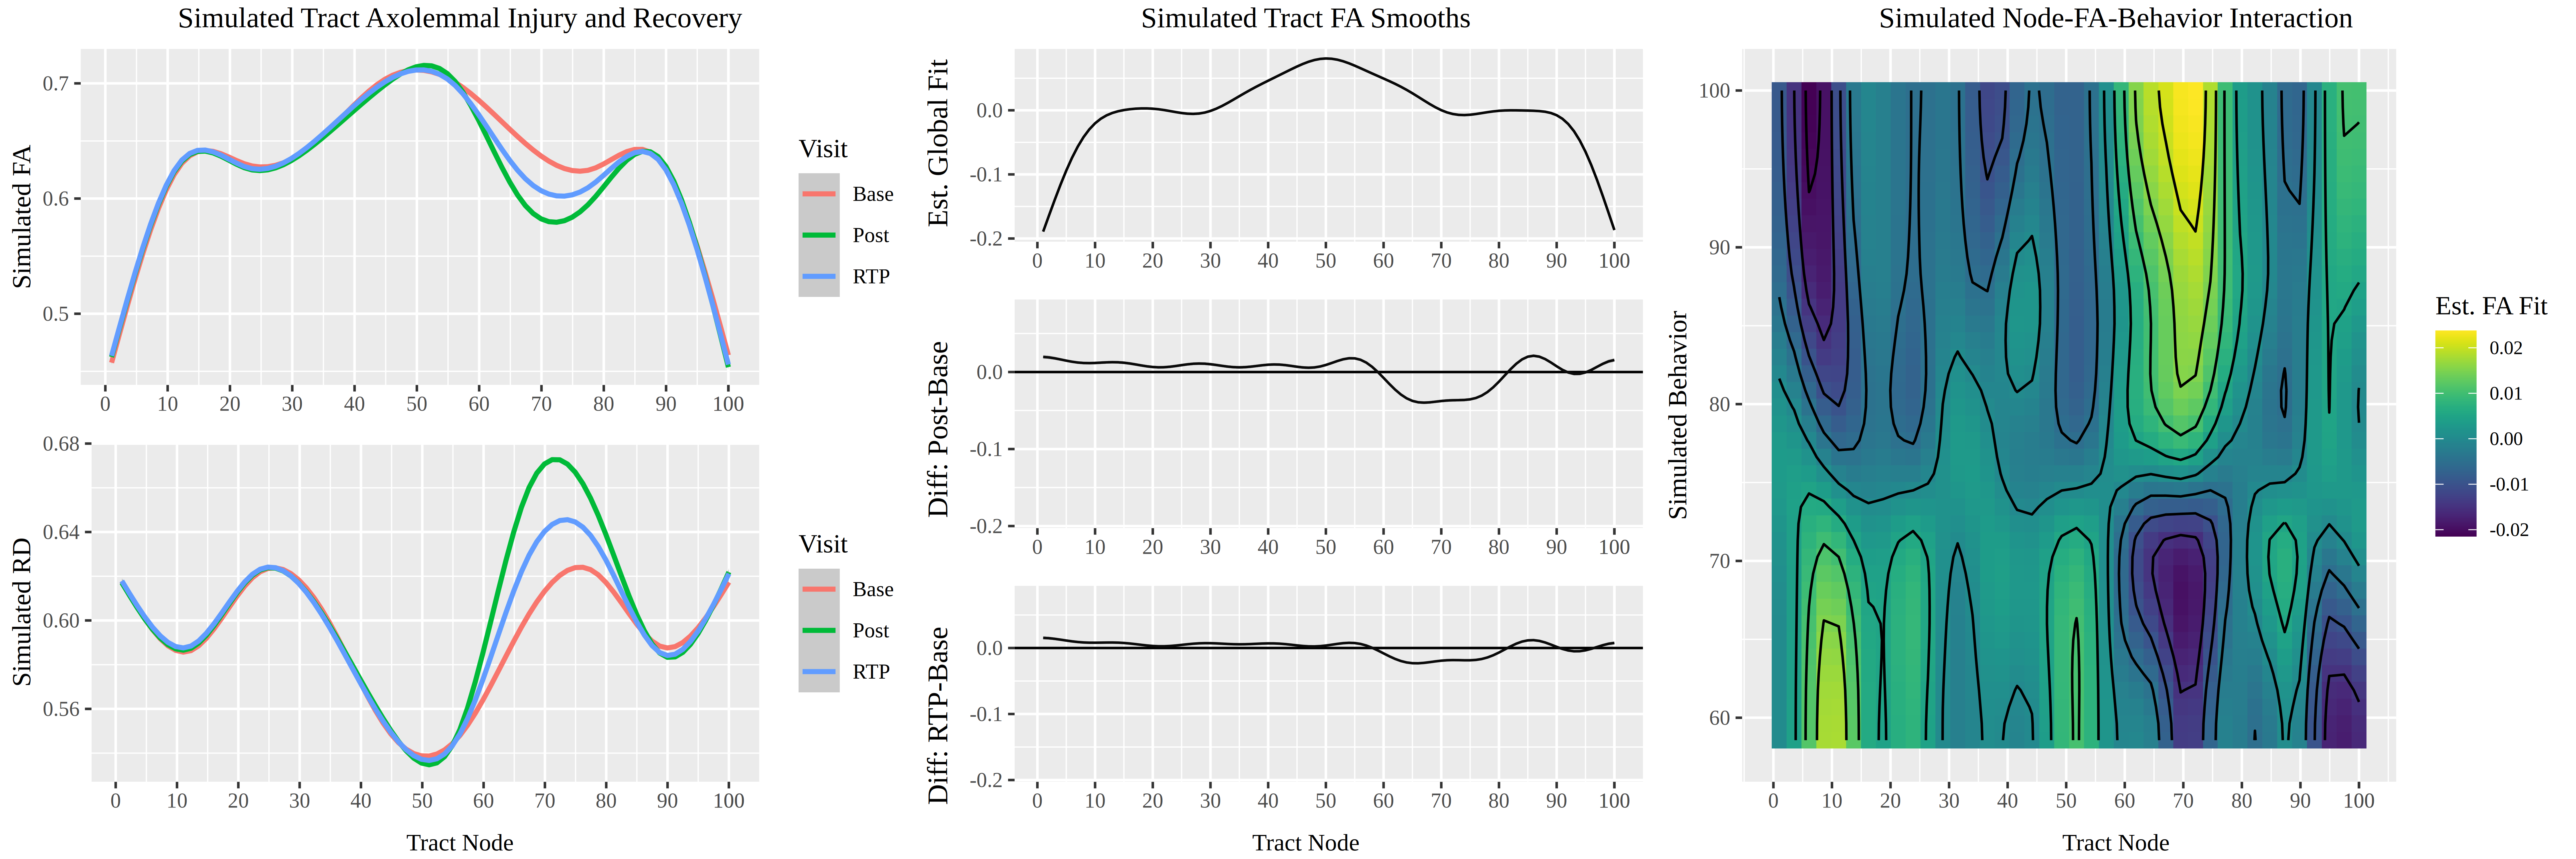
\includegraphics[scale=0.425]{fig_hypotheses.png}}
	\caption{Simulated data to relate hypotheses to PyAFQ-derived tract profiles and GAM smooths, tensor products. \textbf{Left:} simulated PyAFQ tract profiles of FA (top) and RD (bottom) at three visits: baseline (Red), post-concussion (Green), and return-to-play (Blue). Injury resulted in decreased FA values for nodes 60-80 at Post (top), and FA values are mostly (but not entirely) recovered to Base values by RTP. These FA changes relate to corresponding changes in RD (bottom). \textbf{Middle:} smooths produced by a hierarchical generalized additive model of the tract FA profiles across all visits. The overarching curvature of the tract profile is captured as a main effect in the global fit smooth (top). FA values between nodes 60-80 are lower in Post than Base as evidenced in the difference smooth (middle), and these values are partially recovered at RTP (bottom). \textbf{Right:} a simulated interaction between tract FA values and behavioral response modeled with a tensor product interaction smooth. An interaction between behavior and FA values is present in the region of nodes 60-80: higher behavioral values are associated with higher FA values (yellow) while lower behavioral values are related to lower FA values in the same region (blue). Third-order polynomial splines were used to simulate the tract profiles, and behavioral values were shifted by the smallest FA values among the injured nodes. Tract Node = subregion of a segmented white matter tract. FA = fractional anisotropy, RD = radial diffusivity. Base = baseline, Post = post-concussion, RTP = return-to-play.}
	\label{fig:intro-hyp}
\end{figure}


\section{Methods}
\label{sec:meth}

\subsection{Participants}
\label{ssec:meth-part}
Participants were recruited from men's football and women's soccer programs at the University of Nebraska-Lincoln, resulting in the enrollment of 69 (9 female, age = 19.36 $\pm$1.67, range = 17-24) National Collegiate Athletic Association (NCAA) athletes. Additional demographic metrics (e.g. race, ethnicity, SES) are omitted to protect participant confidentiality as University athletes are public figures and identification may cause deleterious consequences. Due to the limited number of females, and the sport-sex confound, we combined all participants into a single group. Institutional Review Board approval was obtained at the outset of the study, and prior to beginning experimental procedures participants completed informed consent and assent. Magnetic Resonant Imaging (MRI) and clinical assessment (ImPACT) data were acquired during three sessions: enrollment at the beginning of the season (baseline, Base), within 48 hours of diagnosed concussion (post-concussion, Post), and prior to return-to-play (RTP). As MRI and ImPACT (below) data were gathered separately, a number of participants did not contribute MRI and/or ImPACT data across one or more of the sessions. This resulted in the following final session counts: Base = 67 MRI (9 female), 61 ImPACT (5 female), Post = 65 MRI (8 female), 48 ImPACT (3 female), and RTP = 56 MRI (7 female), 32 ImPACT (2 female).

% TODO: provide average time between Post and RTP
% TODO: reformat final count? Perhaps a table.

\subsection{ImPACT}
\label{ssec:meth-imp}
We assessed self-reported symptoms and cognitive performance using the Immediate Post-Concussion Assessment and Cognitive Testing (ImPACT), one of the most widely used tools for evaluating concussions \parencite{lovell2005ImPACT200540,dessy2017ReviewAssessmentScales}. Self-reported symptoms were measured with the 22-item Post-Concussion Symptom Scale within ImPACT \parencite{lovell2006MeasurementSymptomsFollowing}. Cognitive performance was assessed through five composite scores derived from ImPACT's computerized neurocognitive tests: verbal memory, visual memory, visual-motor processing speed, impulse control, and reaction time \parencite{lovell2005ImPACT200540}. These assessments were conducted in collaboration with clinicians from our Department of Athletic Medicine and were administered to participants at Base, Post, and throughout their recovery, with the participant's final assessment serving as RTP.


\subsection{MRI Protocol}
\label{ssec:meth-mri}
Magnetic Resonance Imaging data were collected on a 3-Tesla Siemens MAGNETOM Skyra scanner at the Center for Brain, Behavior and Biology (University of Nebraska-Lincoln) utilizing a 20-channel coil. For each of three sessions (Base, Post, and RTP), participants contributed T1 and diffusion weighted images (T1w, DWI). T1w Multi-Echo Magnetization Prepared - RApid GRadient Echo (MEMP-RAGE) structural scans were acquired with the following parameters: TR = 2530 ms, TE = 1.69, 3.55, 5.41, and 7.27 ms, flip angle = 7$^{\circ}$, voxel size = 1 mm$^3$, FoV = 256 $\times$ 256, slices = 176 interleaved. DWI scans were acquired via TR = 3000 ms, TE = 95 ms, flip angle = 90$^{\circ}$, voxel size = 1.719 $\times$ 1.719 $\times$ 2.4 mm$^3$, 134 slices, multi-band acceleration factor = 3, directions = 128, bandwidth = 1500 Hz/Px, shells = 1 (b-value = 1000 s/mm$^2$), reference volumes = 6 (b-values = 0 s/mm$^2$; b$_0$). A set of field maps for the DWI scans were collected using the same acquisition direction (anterior-posterior; AP) and reversed (posterior-anterior; PA).


\subsection{MRI Data Processing}
\label{ssec:meth-mri-proc}
Preprocessing and modeling of the DWI data were conducted using FSL v6.0 \parencite{jenkinson2012Fsl} and PyAFQ v1.3.6 \parencite{kruper2021EvaluatingReliabilityHuman,yeatman2012TractProfilesWhite}. First, b$_0$ volumes and acquisition parameters were extracted and combined from the AP and PA field maps, and \lstinline{topup} used the resulting AP-PA b$_0$ file to calculate a distortion correction matrix. Next, a brain mask was constructed via \lstinline{bet}, and then preprocessing of the DWI data was conducted with \lstinline{eddy_openmp}, which incorporated the distortion correction matrix, brain mask, and a volume-acquisition parameter mapping index to produce motion- and distortion-corrected diffusion images.

Whole-brain tractography was computed from the preprocessed DWI by PyAFQ. Constrained spherical deconvolution was used to derive the fiber orientation distribution function (fODF) of each voxel, where constrained-positivity regularization = 1, minimum amplitude $\tau$ = 0.1, mean gray matter diffusivity = 0.0008, mean CSF diffusivity = 0.003, 600 fODF iterations, and spherical harmonics order = 8. Resulting fODFs of each voxel were then utilized to probabilistically generate fiber maps, using one seed per voxel for each dimension, a maximum turning angle of 30$^\circ$, step size = 0.5 mm, and a length range = 50-250 mm. The resulting fibers were parcellated into individual tracts via \textit{a priori} inclusion (waypoint) and exclusion regions of interest \parencite{wakana2007ReproducibilityQuantitativeTractography}. These tracts were then compared to a fiber probability map \parencite{hua2008TractProbabilityMaps} and any fibers which traverse low-probability spaces were removed from the tract. Further, any fibers with a length 3+ standard deviations from the tract average, or 4+ standard deviations from the average path centroid, were removed as well. Lastly, each tract was then resampled into 100 equidistant nodes (according to a Mahalanobis distance metric) from which averaged diffusion scalars (FA, AD, RD, and MD) were calculated. It was determined upon review of the 28 parcellated tract bundles that bilateral posterior arcuate and vertical occipital tracts were not well identified across all subjects and sessions, accordingly analyses only included the remaining 24 white matter tracts. Finally, as scalar values approach zero at the start and end of tracts due to fiber fanning, fitting the distribution becomes rather problematic. We removed the first and last 10 nodes and were subsequently able to fit the data well, and we note that this clipping of the ends is in addition to that already performed by the PyAFQ software.

% TODO: Cite that CSD, prob tract are better for TBI?


\subsection{Hierarchical Generalized Additive Models Fit Group Tract Scalars}
\label{ssec:meth-gam}
Hierarchical generalized additive models (HGAMs; \cite{pedersen2019HierarchicalGeneralizedAdditive}) allow for model fits at both global and group levels. That is, it is possible to model both the X-Y relationship that is shared across all levels of a factor (global smooth) and differences that factor levels (group smooths) may have from the global smooth. Further, it is not required that each level of smooth (global, group) contain the same `wiggliness' in the X-Y relationships. Separate smooth curves and wiggliness terms at different factor levels of HGAMs is highly relevant in modeling concussion-related changes within white matter tracts, as the global smooth of the tractometric profile (i.e. scalar values across all nodes) can effectively be held constant when modeling potential changes across session, and independent wiggliness terms may capture scalar changes unique to one time point. Further, tensor product interaction terms can be utilized to build multimodal models, investigating the relationship of the tractometric profile with independent metrics such as the ImPACT composite scores. Accordingly, such a model would be capable not only of detecting changes within a tract that result from concussion, but also how such changes relate to clinical assessments. Finally, and critically, HGAMs facilitate conducting longitudinal, whole-brain analyses on tractometric profiles as data from all tracts and across all time points can be included in the same model. Such a specification allows for within-subject pooling of variance across both tract and time. Where modeling individual tracts results in a creeping Type-I error and the corresponding corrections, concussion (and subsequent recovery) may affect multiple tracts within a subject and such shared variance would be lost when investigating tracts individually. By including all tracts and time points, HGAMs have the capability to not only reduce Type-I but also Type-II errors. All GAMs were specified using the \lstinline{mgcv} package version 1.9-1 \parencite{wood2017GeneralizedAdditiveModels} in R version 4.3.3 \parencite{rcoreteam2023LanguageEnvironmentStatistical}.

% TODO: include DWI scalar distribution (and plot) to visualize tractometric profile? Cite a yeatman tractometry paper?


\subsubsection{Whole Brain Longitudinal Difference Model}
\label{sssec:meth-gam-ldi}
To investigate within-tract concussion- and recovery-related FA changes we specified an HGAM to test for Post and RTP tract FA differences from Base. First, we calculated the Post-Base and RTP-Base changes in FA ($\Delta$FA). While including original FA values would be ideal, propagating ordered factors (Base $<$ Post $<$ RTP) across an interaction with another factor (tract) loses the original ordered structure; ordered factors would be necessary to investigate differences from baseline instead of merely the interaction with session. Next, we calculated the session comparison $\times$ tract interaction term as \lstinline{mgcv::bam} does not currently support modeling smooths by factor interactions. $\Delta$FA values were modeled as a function of tract node using thin-plate regression splines (R Code \ref{code:gam-ldi}) and a basis dimensionality of 15 was determined sufficient to fit the tract curves (\lstinline{gam.check(fit_LDI)}). Subjects were treated as a random effect, thereby allowing each subject to have their own intercept across all levels of the factors, the $\Delta$FA distribution was well-fit by a Gaussian distribution with an identity link function, fast Residual Error of Maximum Likelihood (fREML) was used as the smoothing parameter estimation method, and 12 threads were used in the computation (run time $\approx$ 45 minutes). Input data consisted of the 24 tracts with good segmentation across all subjects. Notably, we did not include a global smooth for this model, as the $\Delta$FA profile would differ for each tract, and we specified that each tract would have its own wiggliness term; essentially this is a longitudinal model of FA differences which references model `I' in \textcite{pedersen2019HierarchicalGeneralizedAdditive}.

\begin{equ}[H]
	\begin{lstlisting}
		fit_LDI <- mgcv::bam(
		  delta_fa ~ s(subj_id, by=tract_scan, bs="re") +
		    s(node_id, by=tract_scan, bs="tp", k=15) +
		    tract_name+sess_comp+tract_scan,
		  data=df,
		  family=gaussian(),
		  method="fREML",
		  nthreads=12
		)
	\end{lstlisting}
	\caption{$\Delta$FA values are modeled as a function of tract node with thin-plate regression smooths for each tract, accounting for the within-subject factors of tract and session and using separate wiggliness terms for each tract. \lstinline{delta_fa} = RTP-Base and Post-Base FA differences, \lstinline{subj_id} = subject identifier factor, \lstinline{node_id} = node identifier integer, \lstinline{tract_name} = tract identifier factor, \lstinline{sess_comp} = session comparison factor (RTP-Base, Post-Base), and \lstinline{tract_scan} = interaction of \lstinline{tract_name} and \lstinline{sess_comp}.}
	\label{code:gam-ldi}
\end{equ}


\subsubsection{Tract Longitudinal Scalar Model}
\label{sssec:meth-gam-lgio}
The model specified in R Code \ref{code:gam-ldi} effectively models the entire longitudinal dataset of $\Delta$FA values, allowing for pooling for variance within a subject across tract and session, not requiring a multiple comparison correction for modeling all tracts. But as the $\Delta$FA calculation required data at time points A and B, the analysis was restricted by missing data. As essentially a post-hoc analysis to further interrogate tract differences across session, and also what change in scalar (e.g. increased RD) drove the difference in FA, individual tracts were modeled with a longitudinal HGAM with terms for global and group smooths (R Code \ref{code:gam-lgio}). Tract FA values were fit by a beta distribution with a logit link function, AD and RD values were fit with a Gaussian distribution and identity link function, and a gamma distribution with a logit link function fit the MD values. Subjects were again treated as a random effect, with separate intercepts for each scan (Base, Post, RTP), group smooths were allowed their own wiggliness parameter, and the colinearity of global and group smooths was controlled by the `m' parameter. Such a model is similar to model `GI' in \textcite{pedersen2019HierarchicalGeneralizedAdditive}. Finally, an ordered session factor was included to test for difference in Post and RTP scalar values from Base. Such a model is particularly useful as the test statistic, which describes the flatness of the smooth, provides information about changes from Base values rather than deflections from zero. A model which fits group smooths for each session is provided in Supplemental Materials (Supplemental R code \ref{supp-code:gam-lgi}).

\begin{equ}[H]
	\begin{lstlisting}
		df$scanOF <- factor(df$scan_name, ordered=T)
		fit_LGIO <- mgcv::bam(
		  <scalar> ~ s(subj_id, scan_name, bs="re") +
		    s(node_id, bs="tp", k=15, m=2) +
		    s(node_id, by=scanOF, bs="tp", k=15, m=1),
		  data=df,
		  family=<family>,
		  method="fREML",
		  nthreads=4
		)
	\end{lstlisting}
	\caption{Tract scalars are modeled as a function of tract node with thin-plate regression splines using both global and group (\lstinline{scan_name}) smooths as well as individual group wiggliness. An ordered factor of scan session was used to compare Post and RTP to Base. \lstinline{<scalar>} = relevant DWI metric (AD, RD, MD, or FA), \lstinline{scan_name} = session identifier factor (Base, Post, RTP), \lstinline{scanOf} = ordered factor of \lstinline{scan_name}, \lstinline{<family>} = relevant family and link function for scalar distribution.}
	\label{code:gam-lgio}
\end{equ}


\subsubsection{Tract Longitudinal Scalar Interaction Model}
\label{sssec:meth-gam-lgio-intx}
As noted above, GAMs are capable of modeling higher-dimensional, non-linear interactions through tensor product interaction smooths and hypersurfaces, a property which make them particularly relevant for multimodal research. We used such a model to test whether concussion- and recovery-related changes in tract scalars related to changes in ImPACT composite and total symptom scores (R code \ref{code:gam-lgio-intx}), thereby potentially linking damage within a specific region of a tract to changes in assessment metrics. Tract scalars were modeled as a function of both tract node and ImPACT measure, and the node-ImPACT interaction term was specified such that each session (Base, Post, RTP) would have a different scalar-node-ImpACT interaction surface. We note the decrease in basis dimensionality for the ImPACT measures thin-plate regression splines from the default value, and that fitting the tensor product interaction smooth also benefited from a slightly higher basis dimensions term for the tract node term. Finally, as above (Section \ref{sssec:meth-gam-lgio}), an ordered factor for session was included in order to test whether the Post and RTP interaction surfaces differed from that of Base; a model with separate interaction surfaces is provided in Supplemental Materials (Supplemental R code \ref{supp-code:gam-lgi-intx}).

\begin{equ}[H]
	\begin{lstlisting}
		df$scanOF <- factor(df$scan_name, ordered=T)
		fit_LGIO_intx <- mgcv::bam(
		  <scalar> ~ s(subj_id, scan_name, bs="re") +
		    s(node_id, bs="tp", k=15, m=2) +
		    s(imp_meas, by=scan_name, bs="tp", k=5) +
		    ti(node_id, imp_meas, bs=c"tp","tp"), k=c(20,5), m=1) +
		    ti(
		      node_id, imp_meas, by=scanOF,
		      bs=c("tp","tp"), k=c(20,5), m=1
		    ),
		  data=df,
		  family=<family>,
		  method="fREML",
		  nthreads=4
		)
	\end{lstlisting}
	\caption{Tract scalars are modeled as a function of separate 1D node and ImPACT smooths as well as a 2D tensor product interaction surface, with ordered factors used to compare Post and RTP surfaces to Base. \lstinline{imp_meas} = ImPACT composite or total symptom measure.}
	\label{code:gam-lgio-intx}
\end{equ}


\subsubsection{ImPACT model}
\label{sssec:meth-gam-impact}
The relationship between session (Base, Post, RTP), ImPACT composite metrics (verbal memory, visual memory, visual motor, impulse control, and reaction time), and ImPACT total symptom scores were modeled with GAMs to test for changes across assessment session. As with tract scalar profiles, GAMs were employed as (a) non-linear trends are expected in such metrics and (b) they can model the semi-parametric distributions encountered in several of the metrics. Each ImPACT metric was fit as a function of assessment number, using integer values rather than categorical Base, Post, and RTP (Supplemental R Code \ref{supp-code:gam-impact}); such a specification allowed for modeling evolving changes in assessment metrics rather than comparing main effects across factor levels. Verbal and visual memory composites were converted to proportion scores and modeled with a beta distribution and logit link function, visual motor and reaction time were best fit with Gaussian distributions and identity link functions (despite the skewness), and a negative binomial distribution with log link function fit the impulse control and total symptoms well.

When specifying models, whether with ImPACT or DWI data, model fits were reviewed and assessed via \lstinline{mgcv:gam.check()}, and the selection of competing models was aided by \lstinline{itsadug::compareML()}. Pipeline and statistical code, information about their respective environments, and curated data are available at the project repository: \url{https://github.com/nmuncy/adr_dwi}.


\section{Results}
\label{sec:res}

\subsection{ImPACT Visual Memory, Reaction Time, and Total Symptoms Show Evidence of Injury and Recovery}
\label{ssec:res-imp}
All models of ImPACT metrics (Section \ref{sssec:meth-gam-impact}), except for impulse control, detected a significant interaction between the ImPACT metric and assessment number (Figure \ref{fig:imp-gam}). Visual memory, reaction time, and total symptoms demonstrated patterns consistent with concussion-related deficits at Post and subsequent recovery at RTP (visual memory: $F_{(1.94, 1.99)}$ = 8.59, \textit{p} $<$ .001; reaction time: $F_{(1.91, 1.99)}$ = 6.18, \textit{p} $<$ .01; total symptoms: $F_{(1.98, 1.99)}$ = 28.74, \textit{p} $<$ .0001), and we note that total symptoms at RTP were much lower than at Base (Figure \ref{fig:imp-gam}, bottom right).

Conversely, while verbal memory and visual motor tests indicate significant non-flatness (verbal memory: $F_{(1.82, 1.96)}$ = 4.34, \textit{p} = .028; visual motor: $F_{(1.86, 1.97)}$ = 8.19, \textit{p} $<$ .001), concussion-related changes were not detected between Base and Post and the statistic is driven by RTP values. This pattern possibly reflects a lack of sensitivity at Base and/or practice effects. Finally, impulse control was unchanged (i.e. flat) as a function of assessment ($F_{(1.0, 1)}$ = .003, \textit{p} = .95).

\begin{figure}[H]
	\centering
	\fbox{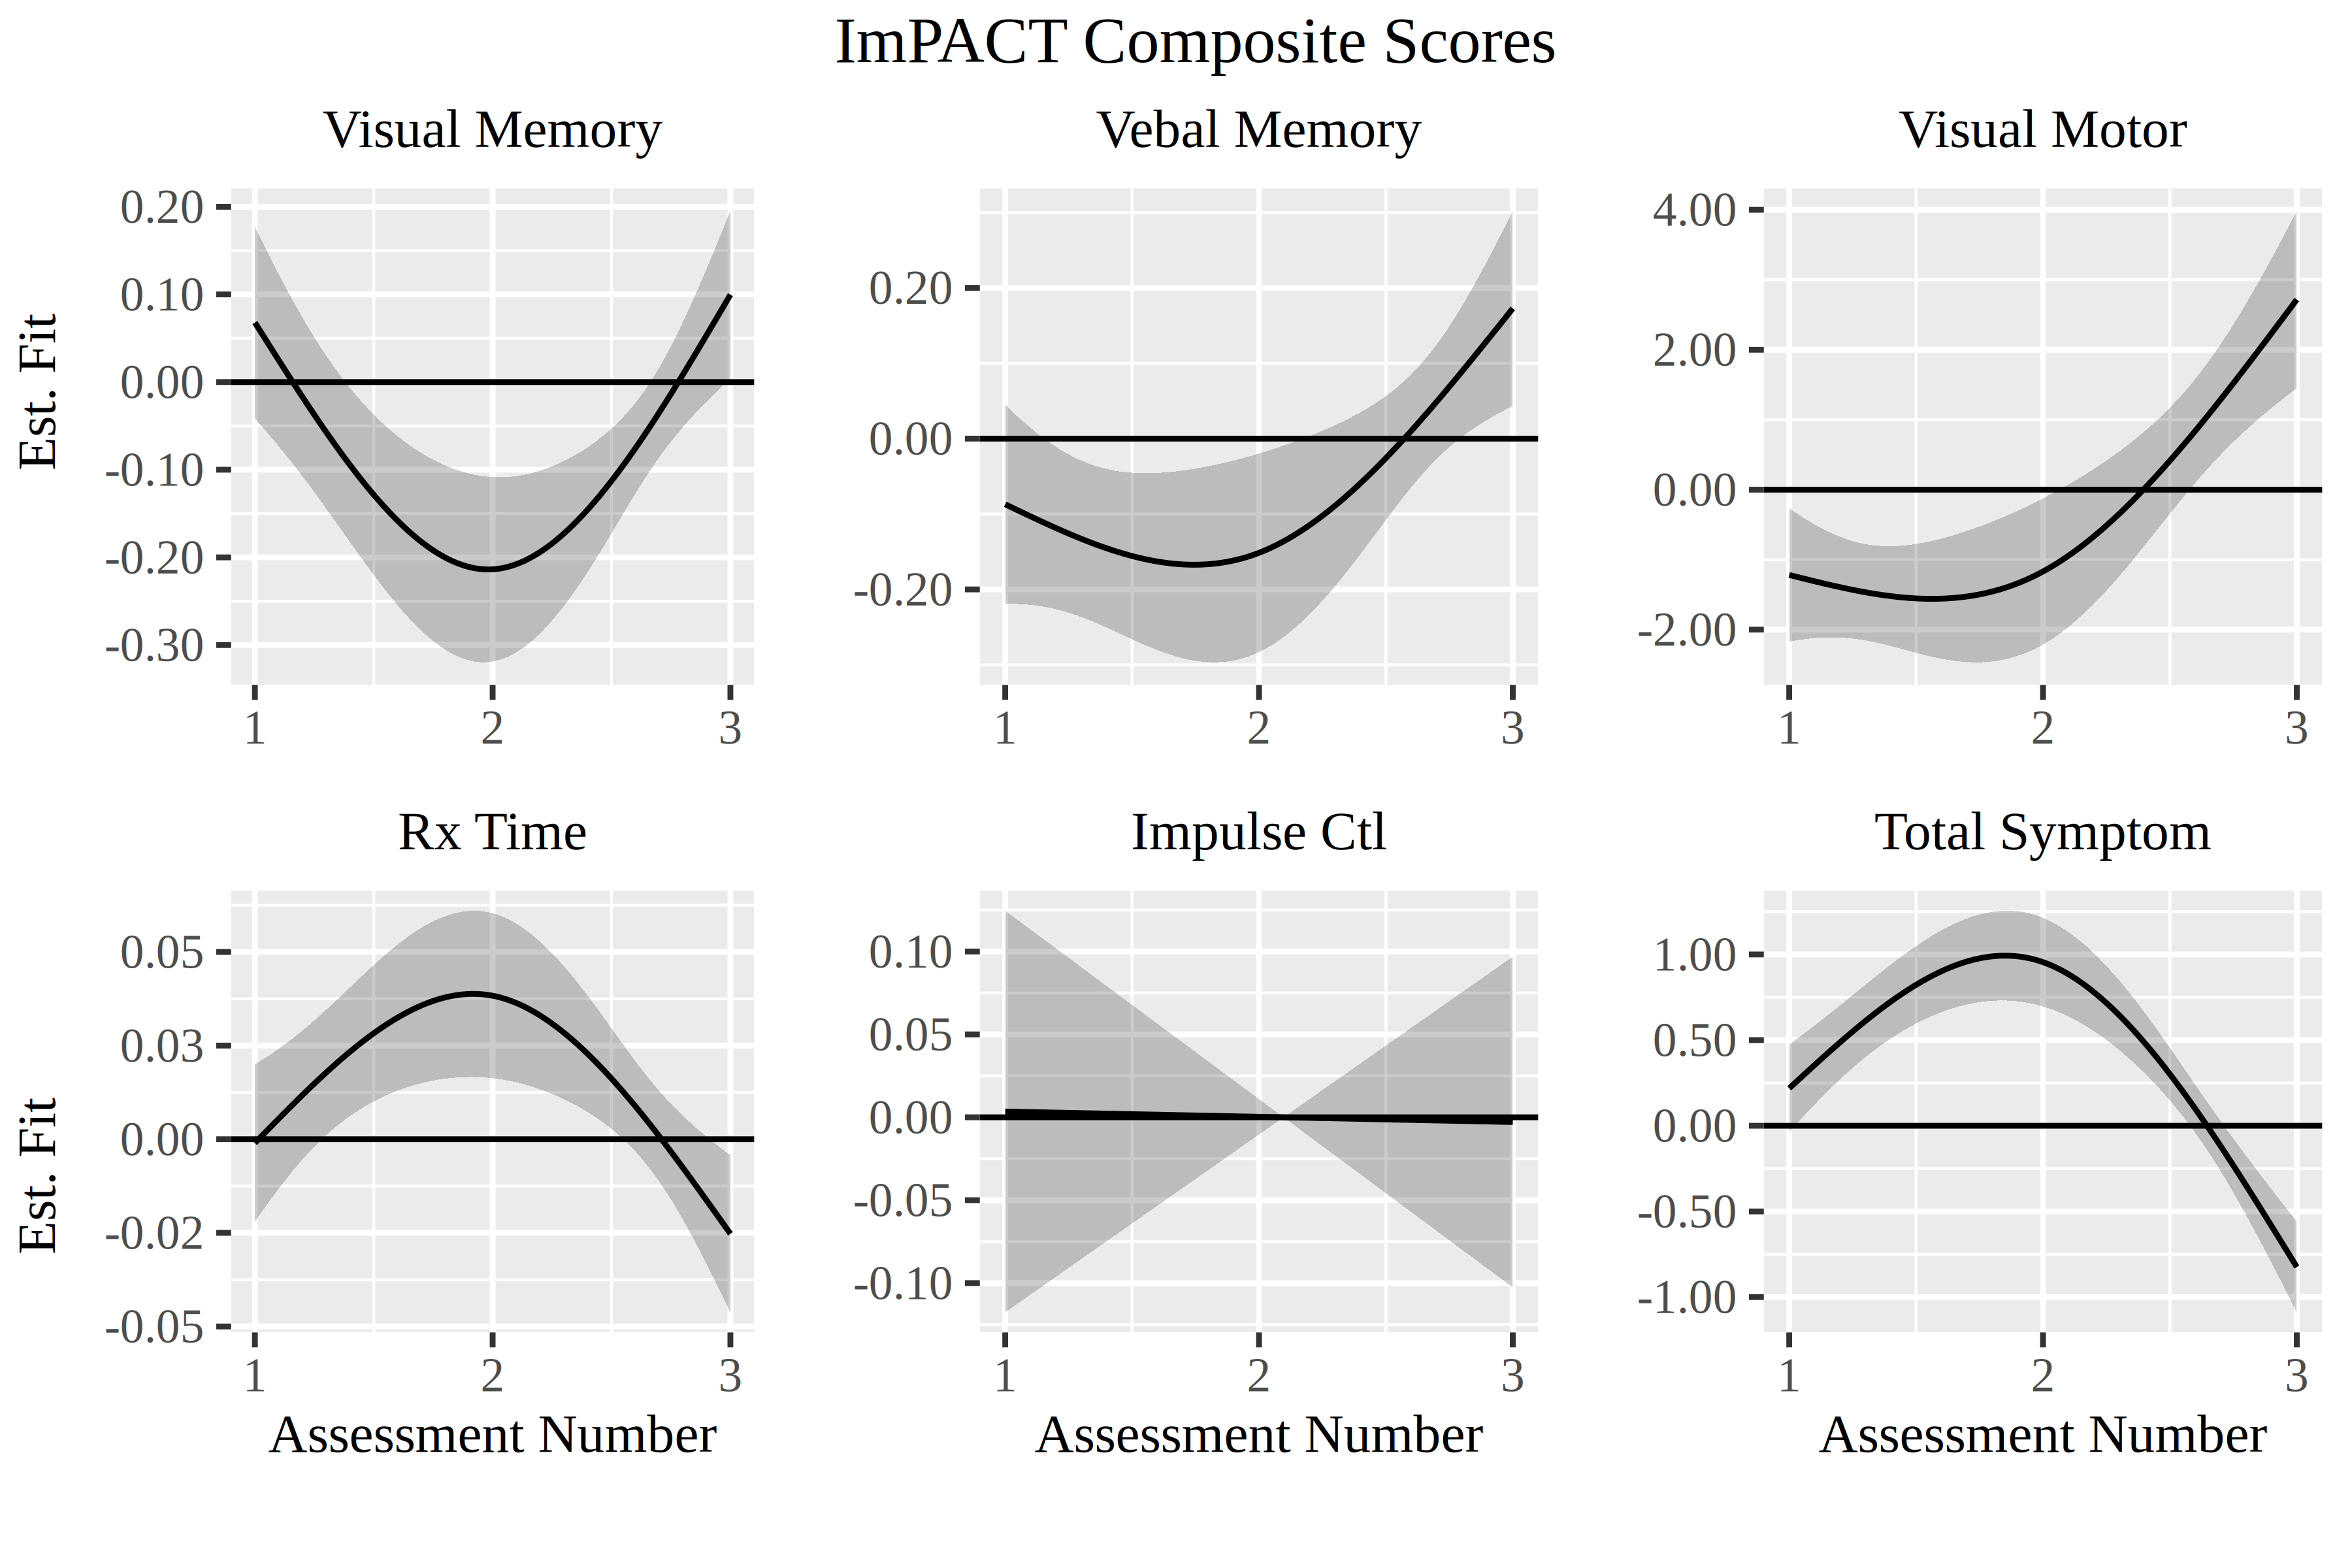
\includegraphics{fig_impact_gam.png}}
	\caption{GAM smooths for ImPACT composite and total symptom scores. Assessment numbers where the confidence interval does not include 0 indicate significant changes. Visual memory, reaction time, and total symptoms showed worsening and then recovery (U-shapes) while verbal memory and visual motor scores were better at assessment 3. Impulse control did not change across assessments. Assessment number 1=Base, 2=Post, 3=RTP. Rx Time = reaction time, Impulse Ctl = impulse control.}
	\label{fig:imp-gam}
\end{figure}


\subsection{Concussion and Recovery in DWI Tractometric Profiles}
\label{ssec:res-dwi-tract}

\subsubsection{Longitudinal Whole-Brain Analyses Implicate Injury in Multiple Tracts}
\label{sssec:res-dwi-tract-wba}
The longitudinal, whole-brain difference model (Section \ref{sssec:meth-gam-ldi}) produced tract difference smooths for Post-Base and RTP-Base $\Delta$FA values (Figure \ref{fig:ldi-gam}, top and middle). Surprisingly, test statistics for all smooths indicated significant non-flatness, suggesting that at least some regions of each tract differed significantly between Base and both Post and RTP (Table \ref{tbl:ldi-gam}). We note that in interpreting GAM coefficients, the magnitude of the effect is equally relevant to the test statistic of non-flatness (F-stat). For instance, when interpreting Figure \ref{fig:ldi-gam}, the callosum orbital (left, green) had a much larger magnitude compared to another, equally `significant' tract (callosum temporal, pink). Nevertheless, it is well established that concussion is associated with negative diagnostic readings \parencite[e.g.][]{klein2019PrevalencePotentiallyClinically}, and we expected to only find changes to scalar values in regions commonly associate with traumatic axonal injury e.g. tracts which decussate through the splenium (here the superior parietal and posterior parietal callosal tracts).

\begin{figure}[H]
	\centering
	\fbox{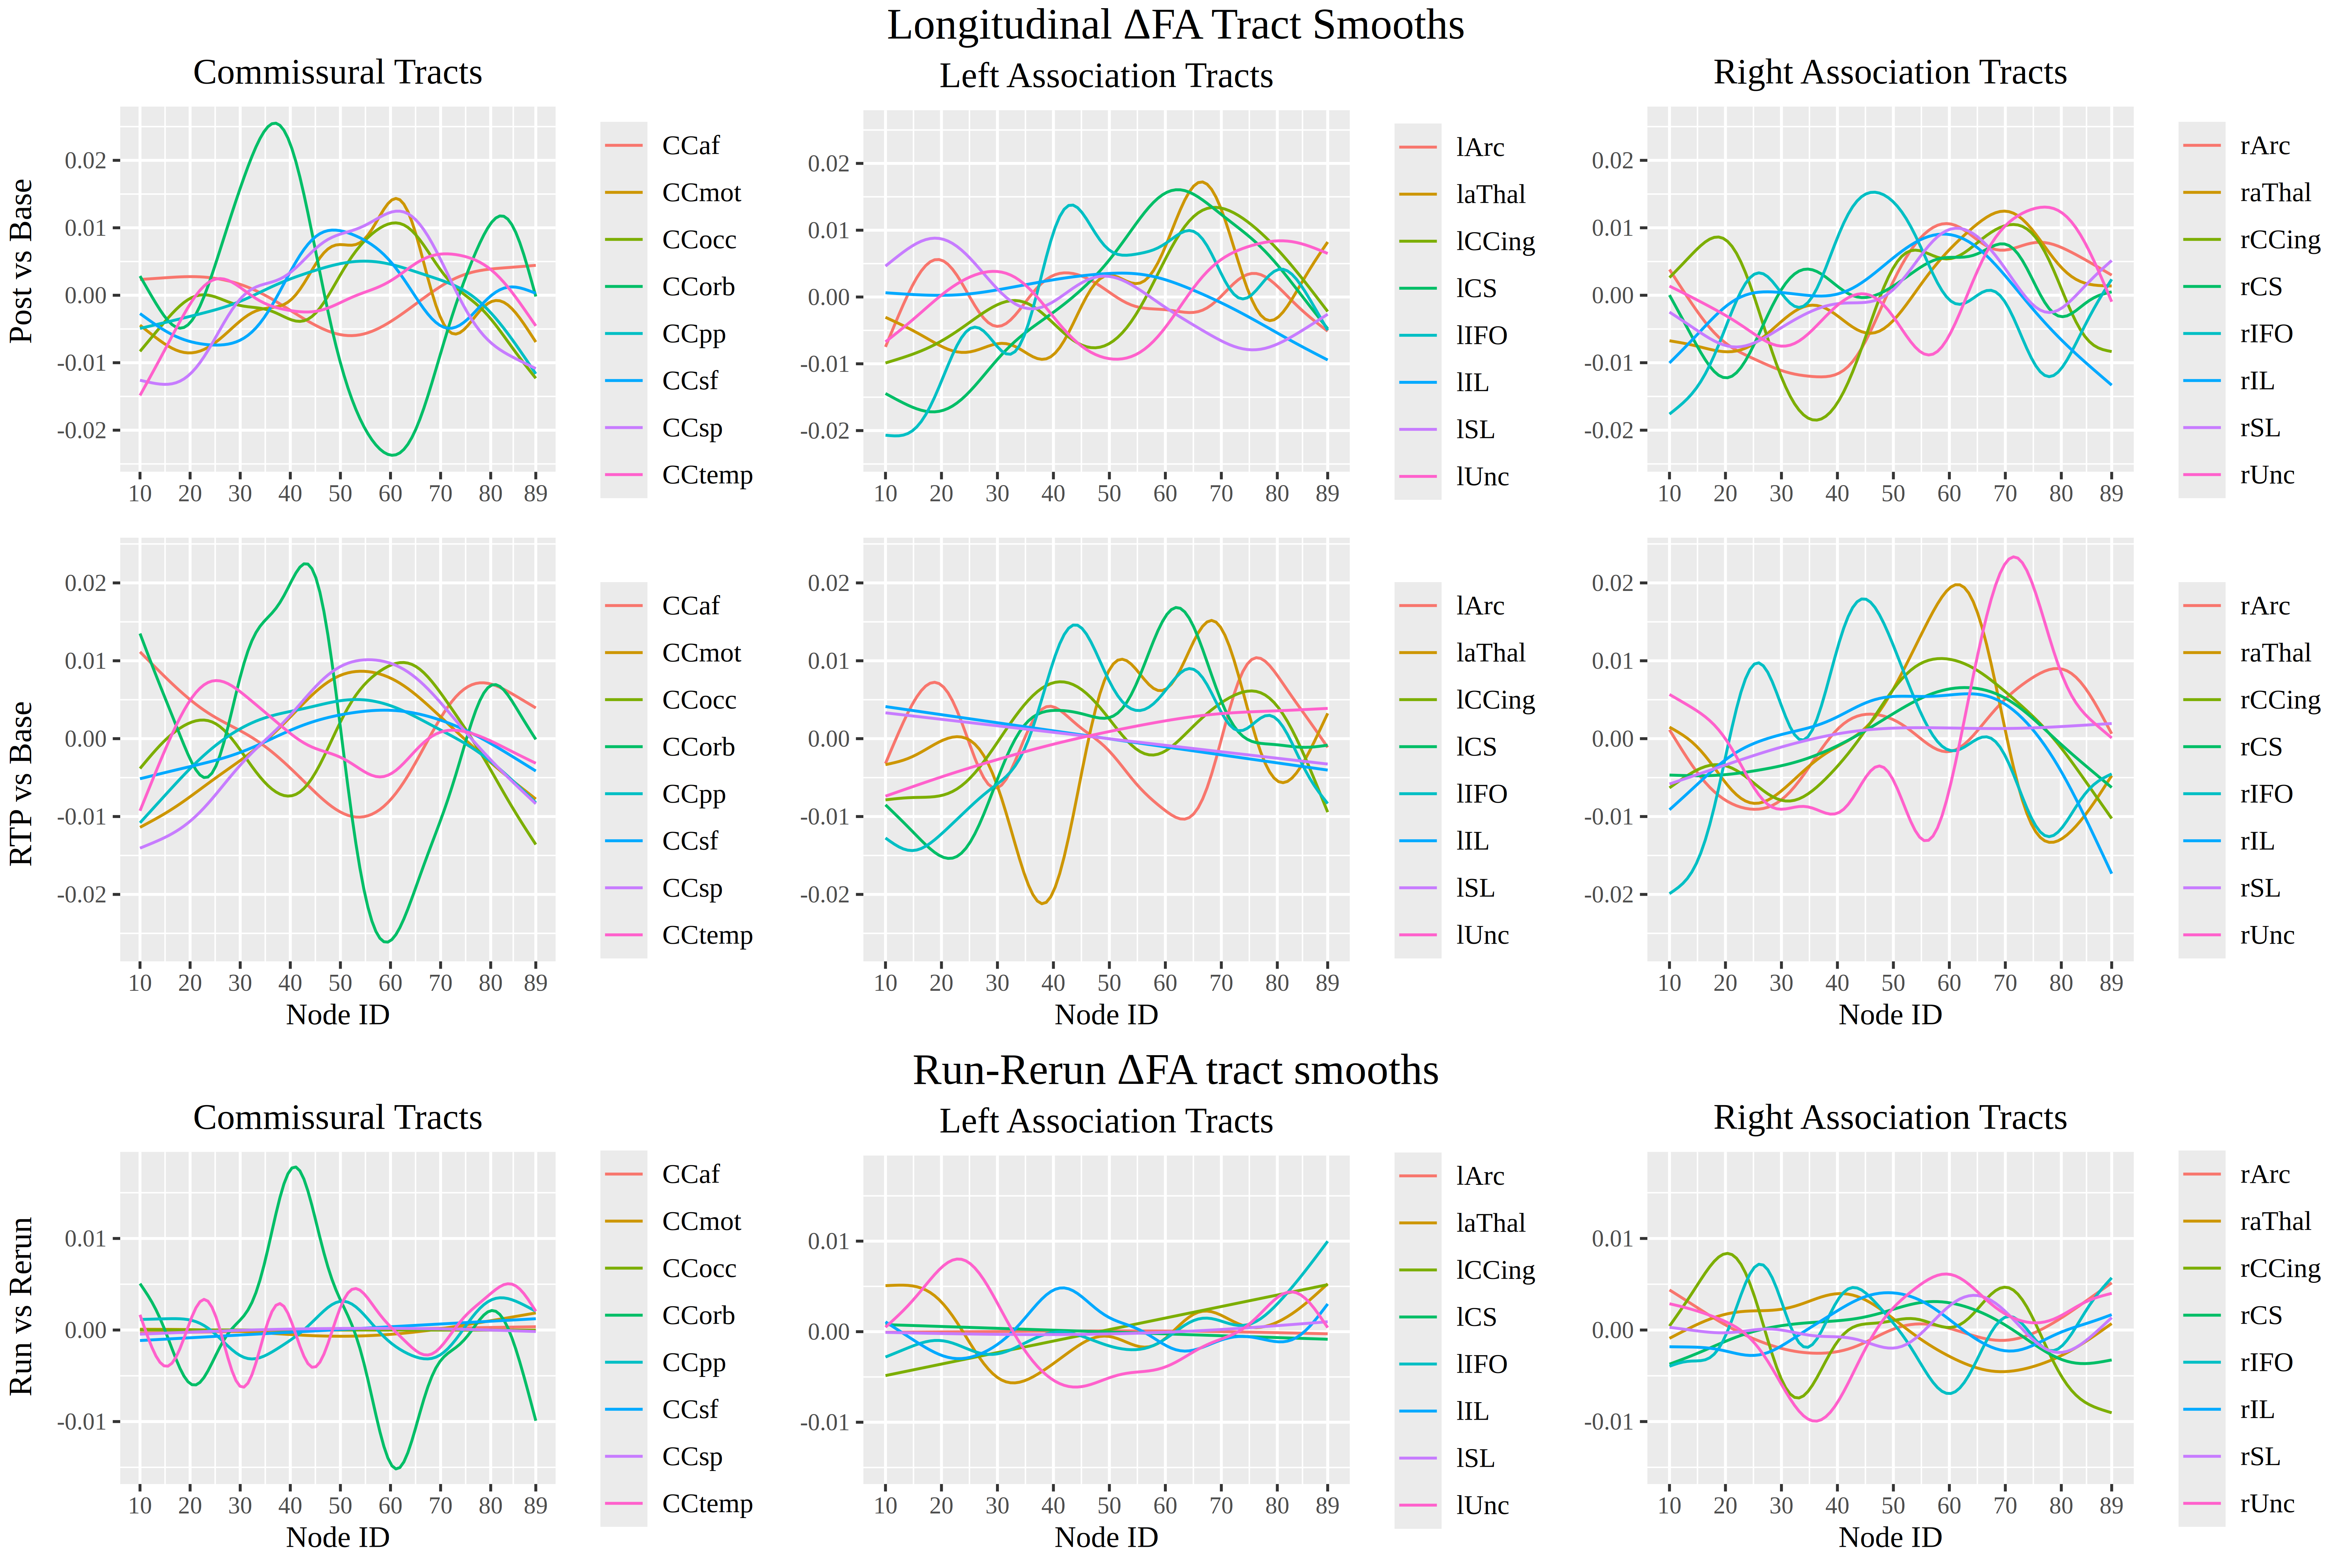
\includegraphics[scale=0.5]{fig_LDI_DI_rerun.png}}
	\caption{HGAM smooths of tract FA differences by node for comparisons against Base (top, middle) and run-rerun (bottom). \textbf{Top}: $\Delta$FA-Node smooths of Post-Base, deflections from zero here may be indicative of concussion-related changes. Middle: $\Delta$FA-Node smooths of RTP-Base, smaller deflections here than Post-Base may be indicative of recovery-related changes (and the converse for greater deflections). \textbf{Bottom}: $\Delta$FA-Node smooths of Run-Rerun, indicative of algorithmic variance by tract. Left: Corpus callosum tracts, middle: left hemisphere tracts, right: right hemisphere tracts. CCaf = anterior forceps, CCmot = motor, CCocc = occipital, CCorb = orbitalis, CCpp = posterior parietal, CCsf = superior frontal, CCsp = superior parietal, CCtemp = temporal. Arc = arcuate, aThal = anterior thalamic, CCing = cingulum (cingulate portion), CS = corticospinal, IFO = inferior fronto-occipital, IL = inferior lateral, SL = superior lateral, Unc = uncinate. Node IDs are counted posterior-anterior or right-left. Confidence intervals were omitted for visual clarity.}
	\label{fig:ldi-gam}
\end{figure}

As tractometry was conducted on each session via PyAFQ, one potential source of variance is algorithmic (i.e. pipeline) run-rerun (test-retest) stability, particularly given our use of probabilistic tractography. Previous work has demonstrated high test-retest reliability metrics for PyAFQ \parencite{kruper2021EvaluatingReliabilityHuman}, which also noted tract-dependent reliability metrics that averaged around 86\%. We note that concussion-related scalar changes may not be as large as 14\%, particularly at the group level due to injury heterogeneity. Nevertheless, we reran tractography on the Base session and calculated Run-Rerun $\Delta$FA values for each subject's tract profiles to quantify the amount of algorithmic variance in our data. The Run-Rerun $\Delta$FA were modeled with a non-longitudinal variant of R Code \ref{code:gam-ldi} (Supplemental R Code \ref{supp-code:gam-di}). Resulting smooths (Figure \ref{fig:ldi-gam}, bottom) illustrate the amount of algorithmic variance that can be expected for each tract, where some tracts have demonstrably high variance (e.g. callosum orbitalis) while others are more stable (superior frontal callosum). Corresponding test statistics identified a number of tracts which did not significantly differ between run and rerun (Table \ref{tbl:ldi-gam}).

\begin{table}[H]
	\scriptsize
	% Please add the following required packages to your document preamble:
% \usepackage[table,xcdraw]{xcolor}
% Beamer presentation requires \usepackage{colortbl} instead of \usepackage[table,xcdraw]{xcolor}
\begin{tabular}{lllll|llll|llll}
 & \multicolumn{4}{c|}{Post-Base} & \multicolumn{4}{c|}{RTP-Base} & \multicolumn{4}{c}{Run-Rerun} \\ \cline{2-13}
Tract & \multicolumn{1}{c}{edf} & \multicolumn{1}{c}{Ref.df} & \multicolumn{1}{c}{F} & \multicolumn{1}{c|}{Sig} & \multicolumn{1}{c}{edf} & \multicolumn{1}{c}{Ref.df} & \multicolumn{1}{c}{F} & \multicolumn{1}{c|}{Sig} & \multicolumn{1}{c}{edf} & \multicolumn{1}{c}{Ref.df} & \multicolumn{1}{c}{F} & \multicolumn{1}{c}{Sig} \\ \hline
\multicolumn{1}{l|}{CCaf} & 4.58 & 5.70 & 5.52 & \textbf{***} & 5.82 & 7.20 & 11.90 & \textbf{***} & 1.00 & 1.00 & 0.34 & \textbf{} \\
\rowcolor[HTML]{C0C0C0}
\multicolumn{1}{l|}{\cellcolor[HTML]{C0C0C0}CCmot} & 9.63 & 11.43 & 9.89 & \textbf{***} & 4.34 & 5.41 & 15.23 & \textbf{***} & 2.27 & 2.83 & 1.84 & \textbf{} \\
\multicolumn{1}{l|}{CCocc} & 7.13 & 8.74 & 9.12 & \textbf{***} & 6.79 & 8.35 & 9.53 & \textbf{***} & 1.00 & 1.01 & \cellcolor[HTML]{FFFFFF}0.00 & \textbf{} \\
\rowcolor[HTML]{C0C0C0}
\multicolumn{1}{l|}{\cellcolor[HTML]{C0C0C0}CCorb} & 9.71 & 11.50 & 30.92 & \textbf{***} & 10.56 & 12.28 & 28.06 & \textbf{***} & 12.01 & 13.35 & 36.29 & \textbf{***} \\
\multicolumn{1}{l|}{CCpp} & 4.35 & 5.42 & 7.62 & \textbf{***} & 3.78 & 4.71 & 9.10 & \textbf{***} & 8.01 & 9.74 & 4.43 & \textbf{***} \\
\rowcolor[HTML]{C0C0C0}
\multicolumn{1}{l|}{\cellcolor[HTML]{C0C0C0}CCsf} & 7.20 & 8.83 & 9.11 & \textbf{***} & 3.15 & 3.94 & 4.77 & \textbf{***} & 1.00 & 1.00 & 3.95 & \textbf{*} \\
\multicolumn{1}{l|}{CCsp} & 7.09 & 8.70 & 20.93 & \textbf{***} & 4.75 & 5.91 & 21.22 & \textbf{***} & 1.43 & 1.74 & 0.34 & \textbf{} \\
\rowcolor[HTML]{C0C0C0}
\multicolumn{1}{l|}{\cellcolor[HTML]{C0C0C0}CCtemp} & 6.40 & 7.89 & 6.61 & \textbf{***} & 6.32 & 7.80 & 4.43 & \textbf{***} & 12.31 & 13.52 & 6.23 & \textbf{***} \\
\multicolumn{1}{l|}{laThal} & 9.98 & 11.76 & 12.34 & \textbf{***} & 10.55 & 12.27 & 15.29 & \textbf{***} & 8.20 & 9.95 & 8.54 & \textbf{***} \\
\rowcolor[HTML]{C0C0C0}
\multicolumn{1}{l|}{\cellcolor[HTML]{C0C0C0}lArc} & 8.59 & 10.37 & 2.67 & \textbf{**} & 9.78 & 11.57 & 6.50 & \textbf{***} & 1.26 & 1.47 & 0.06 & \textbf{} \\
\multicolumn{1}{l|}{lCCing} & 7.17 & 8.79 & 15.00 & \textbf{***} & 6.96 & 8.55 & 6.98 & \textbf{***} & 1.00 & 1.00 & 70.30 & \textbf{***} \\
\rowcolor[HTML]{C0C0C0}
\multicolumn{1}{l|}{\cellcolor[HTML]{C0C0C0}lCS} & 6.41 & 7.90 & 37.00 & \textbf{***} & 8.88 & 10.67 & 15.25 & \textbf{***} & 1.00 & 1.00 & 1.82 & \textbf{} \\
\multicolumn{1}{l|}{lIFO} & 10.64 & 12.35 & 18.33 & \textbf{***} & 9.48 & 11.28 & 13.52 & \textbf{***} & 7.20 & 8.83 & 7.73 & \textbf{***} \\
\rowcolor[HTML]{C0C0C0}
\multicolumn{1}{l|}{\cellcolor[HTML]{C0C0C0}lIL} & 3.38 & 4.22 & 7.15 & \textbf{***} & 1.01 & 1.02 & 11.67 & \textbf{***} & 7.83 & 9.54 & 4.46 & \textbf{***} \\
\multicolumn{1}{l|}{lSL} & 6.58 & 8.11 & 8.14 & \textbf{***} & 1.00 & 1.01 & 7.67 & \textbf{***} & 1.61 & 1.99 & 0.88 & \textbf{} \\
\rowcolor[HTML]{C0C0C0}
\multicolumn{1}{l|}{\cellcolor[HTML]{C0C0C0}lUnc} & 6.45 & 7.95 & 10.78 & \textbf{***} & 2.00 & 2.50 & 10.26 & \textbf{***} & 8.57 & 10.34 & 15.05 & \textbf{***} \\
\multicolumn{1}{l|}{raThal} & 7.32 & 8.97 & 12.45 & \textbf{***} & 9.06 & 10.86 & 17.64 & \textbf{***} & 5.68 & 7.04 & 9.47 & \textbf{***} \\
\rowcolor[HTML]{C0C0C0}
\multicolumn{1}{l|}{\cellcolor[HTML]{C0C0C0}rArc} & 7.33 & 8.97 & 17.97 & \textbf{***} & 6.94 & 8.53 & 7.59 & \textbf{***} & 5.41 & 6.71 & 5.30 & \textbf{***} \\
\multicolumn{1}{l|}{rCCing} & 9.41 & 11.21 & 18.11 & \textbf{***} & 6.07 & 7.50 & 11.80 & \textbf{***} & 10.61 & 12.33 & 14.86 & \textbf{***} \\
\rowcolor[HTML]{C0C0C0}
\multicolumn{1}{l|}{\cellcolor[HTML]{C0C0C0}rCS} & 8.95 & 10.75 & 6.66 & \textbf{***} & 4.17 & 5.19 & 7.53 & \textbf{***} & 5.18 & 6.43 & 6.69 & \textbf{***} \\
\multicolumn{1}{l|}{rIFO} & 10.10 & 11.87 & 15.38 & \textbf{***} & 10.60 & 12.31 & 16.69 & \textbf{***} & 11.49 & 13.01 & 8.77 & \textbf{***} \\
\rowcolor[HTML]{C0C0C0}
\multicolumn{1}{l|}{\cellcolor[HTML]{C0C0C0}rIL} & 5.74 & 7.10 & 12.47 & \textbf{***} & 4.99 & 6.20 & 11.56 & \textbf{***} & 6.18 & 7.63 & 5.82 & \textbf{***} \\
\multicolumn{1}{l|}{rSL} & 7.32 & 8.97 & 7.52 & \textbf{***} & 2.30 & 2.87 & 3.64 & \textbf{*} & 7.45 & 9.11 & 2.92 & \textbf{**} \\
\rowcolor[HTML]{C0C0C0}
\multicolumn{1}{l|}{\cellcolor[HTML]{C0C0C0}rUnc} & 8.43 & 10.19 & 11.34 & \textbf{***} & 10.18 & 11.94 & 18.80 & \textbf{***} & 8.62 & 10.40 & 16.32 & \textbf{***}
\end{tabular}

	\caption{Longitudinal whole-brain HGAM statistics for tract smooths. Significant non-flatness was detected for all difference smooths in the longitudinal concussion model (Post-Base, RTP-Base), and a number of tracts did not show significant differences between multiple runs of the tractography pipeline (Run-Rerun) e.g. CCsp. Post-Base = FA difference between Post and Base, RTP-Base = FA difference between RTP and Base, Run-Rerun = FA difference between multiple runs of PyAFQ. edf = effective degrees of freedom, F = F-statistic, Sig = significance. *** = p$<$.001, ** = p$<$.01, * = p$<$.05.}
	\label{tbl:ldi-gam}
\end{table}

Together, these whole-brain longitudinal and run-rerun analyses of tract FA changes offer support of our first hypothesis that concussion-related changes would be detected in the posterior callosum. Significant Post-Base and RTP-Base differences were detected in the superior posterior region of corpus callosum (CCsp) by the longitudinal concussion HGAM while, importantly, such differences were not driven by algorithmic variance. Further, non-trivial difference magnitudes above and beyond any potential algorithmic variance were detected in a number of callosal and ipsilateral tracts, discussed below.


\subsubsection{Tract-Specific Analyses Determine Source of FA Changes}
\label{sssec:res-dwi-tract-tsa}
\textit{Corpus Callosum Results}. Close inspection of the whole-brain longitudinal and run-rerun results implicated four callosal tracts that demonstrated concussion-related statistics that were practically significant: superior parietal, superior frontal, motor, and orbital. Each of these tracts had non-trivial partial effect magnitudes as well as $\Delta$FA that were greater than was explained by algorithmic variance alone. As FA differences can be driven by changes in AD \textit{or} RD, which are related to different injury sequelae, we modeled FA, MD, AD, and RD for each of these tracts, testing for Post and RTP differences from Base (R Code \ref{code:gam-lgio}). This analysis also had an additional benefit: where $\Delta$FA calculations require data at both time points for subtraction, these longitudinal models of a single tract and scalar had a reduced factor structure such that we were able to use scalars as the predicted values, thereby increasing the number of participants in the model.

Statistical significance was detected for each scalar's smooths (Table \ref{tbl:lgio-gam-cc}), and inspection of these smooths revealed three patterns of injury (Figure \ref{fig:lgio-gam-cc}). First, the Post-Base and RTP-Base FA differences appear to be constant for the superior parietal tract (Figure \ref{fig:lgio-gam-cc}, A), where FA values about nodes 50-60 are increased relative to Base and this FA difference is seemingly driven by a decreased RD. Such a pattern recovery is consistent with cytotoxic edema, particularly given the lack of change in AD. Second, evidence of recovery is apparent in the superior frontal tract (Figure \ref{fig:lgio-gam-cc}, B), where FA values about node 50 are elevated at Post relative to Base, and RD values decreased, a pattern that is again consistent with edema. Both scalars return to near-Base values at RTP, seemingly indicative of healing.

\begin{table}[H]
	\scriptsize
	% Please add the following required packages to your document preamble:
% \usepackage{multirow}
% \usepackage[table,xcdraw]{xcolor}
% Beamer presentation requires \usepackage{colortbl} instead of \usepackage[table,xcdraw]{xcolor}

\begin{tabular}{llll|ll|ll|ll}
 &  & \multicolumn{2}{c|}{FA} & \multicolumn{2}{c|}{MD} & \multicolumn{2}{c|}{AD} & \multicolumn{2}{c}{RD} \\ \cline{3-10}
Tract & Smooth & \multicolumn{1}{c}{edf} & \multicolumn{1}{c|}{F} & \multicolumn{1}{c}{edf} & \multicolumn{1}{c|}{F} & \multicolumn{1}{c}{edf} & \multicolumn{1}{c|}{F} & \multicolumn{1}{c}{edf} & \multicolumn{1}{c}{F} \\ \hline
 & \multicolumn{1}{l|}{Global} & 13.96 & 2750.34 & 13.29 & 256.90 & 13.96 & 4077.09 & 13.83 & 636.96 \\
 & \multicolumn{1}{l|}{\cellcolor[HTML]{C0C0C0}O.Post} & \cellcolor[HTML]{C0C0C0}8.21 & \cellcolor[HTML]{C0C0C0}9.66 & \cellcolor[HTML]{C0C0C0}9.46 & \cellcolor[HTML]{C0C0C0}12.01 & \cellcolor[HTML]{C0C0C0}6.94 & \cellcolor[HTML]{C0C0C0}3.76 & \cellcolor[HTML]{C0C0C0}8.95 & \cellcolor[HTML]{C0C0C0}11.00 \\
\multirow{-3}{*}{CCsp} & \multicolumn{1}{l|}{O.RTP} & 8.10 & 11.02 & 9.30 & 12.57 & 6.29 & 3.02 & 9.04 & 11.67 \\
\rowcolor[HTML]{EFEFEF}
\cellcolor[HTML]{EFEFEF} & \multicolumn{1}{l|}{\cellcolor[HTML]{EFEFEF}Global} & 13.95 & 582.48 & 13.80 & 2762.05 & 13.97 & 4854.79 & 13.82 & 513.35 \\
\rowcolor[HTML]{C0C0C0}
\cellcolor[HTML]{EFEFEF} & \multicolumn{1}{l|}{\cellcolor[HTML]{C0C0C0}O.Post} & 8.99 & 4.70 & 6.23 & 2.68 & 6.29 & 1.14 & 8.53 & 5.78 \\
\rowcolor[HTML]{EFEFEF}
\multirow{-3}{*}{\cellcolor[HTML]{EFEFEF}CCsf} & \multicolumn{1}{l|}{\cellcolor[HTML]{EFEFEF}O.RTP} & 7.01 & 3.51 & 8.33 & 6.03 & 6.97 & 1.81 & 7.71 & 5.81 \\
\rowcolor[HTML]{FFFFFF}
\cellcolor[HTML]{FFFFFF} & \multicolumn{1}{l|}{\cellcolor[HTML]{FFFFFF}Global} & 13.95 & 538.33 & 13.86 & 3284.55 & 13.98 & 5804.04 & 13.62 & 501.66 \\
\rowcolor[HTML]{C0C0C0}
\cellcolor[HTML]{FFFFFF} & \multicolumn{1}{l|}{\cellcolor[HTML]{C0C0C0}O.Post} & 8.88 & 4.34 & 8.91 & 6.27 & 6.37 & 2.00 & 8.91 & 4.87 \\
\rowcolor[HTML]{FFFFFF}
\multirow{-3}{*}{\cellcolor[HTML]{FFFFFF}CCmot} & \multicolumn{1}{l|}{\cellcolor[HTML]{FFFFFF}O.RTP} & 8.41 & 8.05 & 8.72 & 8.74 & 6.41 & 1.26 & 8.28 & 8.54 \\
\rowcolor[HTML]{EFEFEF}
\cellcolor[HTML]{EFEFEF} & \multicolumn{1}{l|}{\cellcolor[HTML]{EFEFEF}Global} & 13.01 & 500.23 & 10.65 & 94.12 & 12.52 & 549.89 & 12.27 & 94.55 \\
\rowcolor[HTML]{C0C0C0}
\cellcolor[HTML]{EFEFEF} & \multicolumn{1}{l|}{\cellcolor[HTML]{C0C0C0}O.Post} & 10.48 & 9.31 & 7.15 & 3.24 & 8.15 & 3.00 & 9.13 & 6.58 \\
\rowcolor[HTML]{EFEFEF}
\multirow{-3}{*}{\cellcolor[HTML]{EFEFEF}CCorb} & \multicolumn{1}{l|}{\cellcolor[HTML]{EFEFEF}O.RTP} & 11.47 & 12.39 & 11.92 & 16.88 & 10.86 & 11.00 & 11.95 & 16.50
\end{tabular}

	\caption{Tract-specific HGAM statistics for DWI scalars of select tracts. Separate models were conducted for each scalar of each tract, fitting both the Global curvature and Group (Post, RTP) differences from Base. O.Post/RTP = Post/RTP group smooth as an ordered factor (relative to Base). edf = effective degrees of freedom, F = F-statistic, Sig = significance. *** = p$<$.001, ** = p$<$.01, * = p$<$.05.}
	\label{tbl:lgio-gam-cc}
\end{table}

Finally, two tracts appear to worsen between Post and RTP: the motor and orbital tracts (Figure \ref{fig:lgio-gam-cc}, C \& D). As with the other tracts, the motor portion of corpus callosum appears to have inflated FA values relative to Base about node 50, driven by decreased RD. Instead of constancy or recovery, however, the difference in scalar values spreads leftward (nodes 40-50). Conversely, the orbitalis portion has a decrease in FA values around node 60 (and increased RD) in Post relative to Base, a difference which increases in magnitude by RTP. This pattern, in opposition to those in panels A-C, is likely reflective of axolemmal permeability rather than cytotoxic edema.

\begin{figure}[H]
	\centering
	\fbox{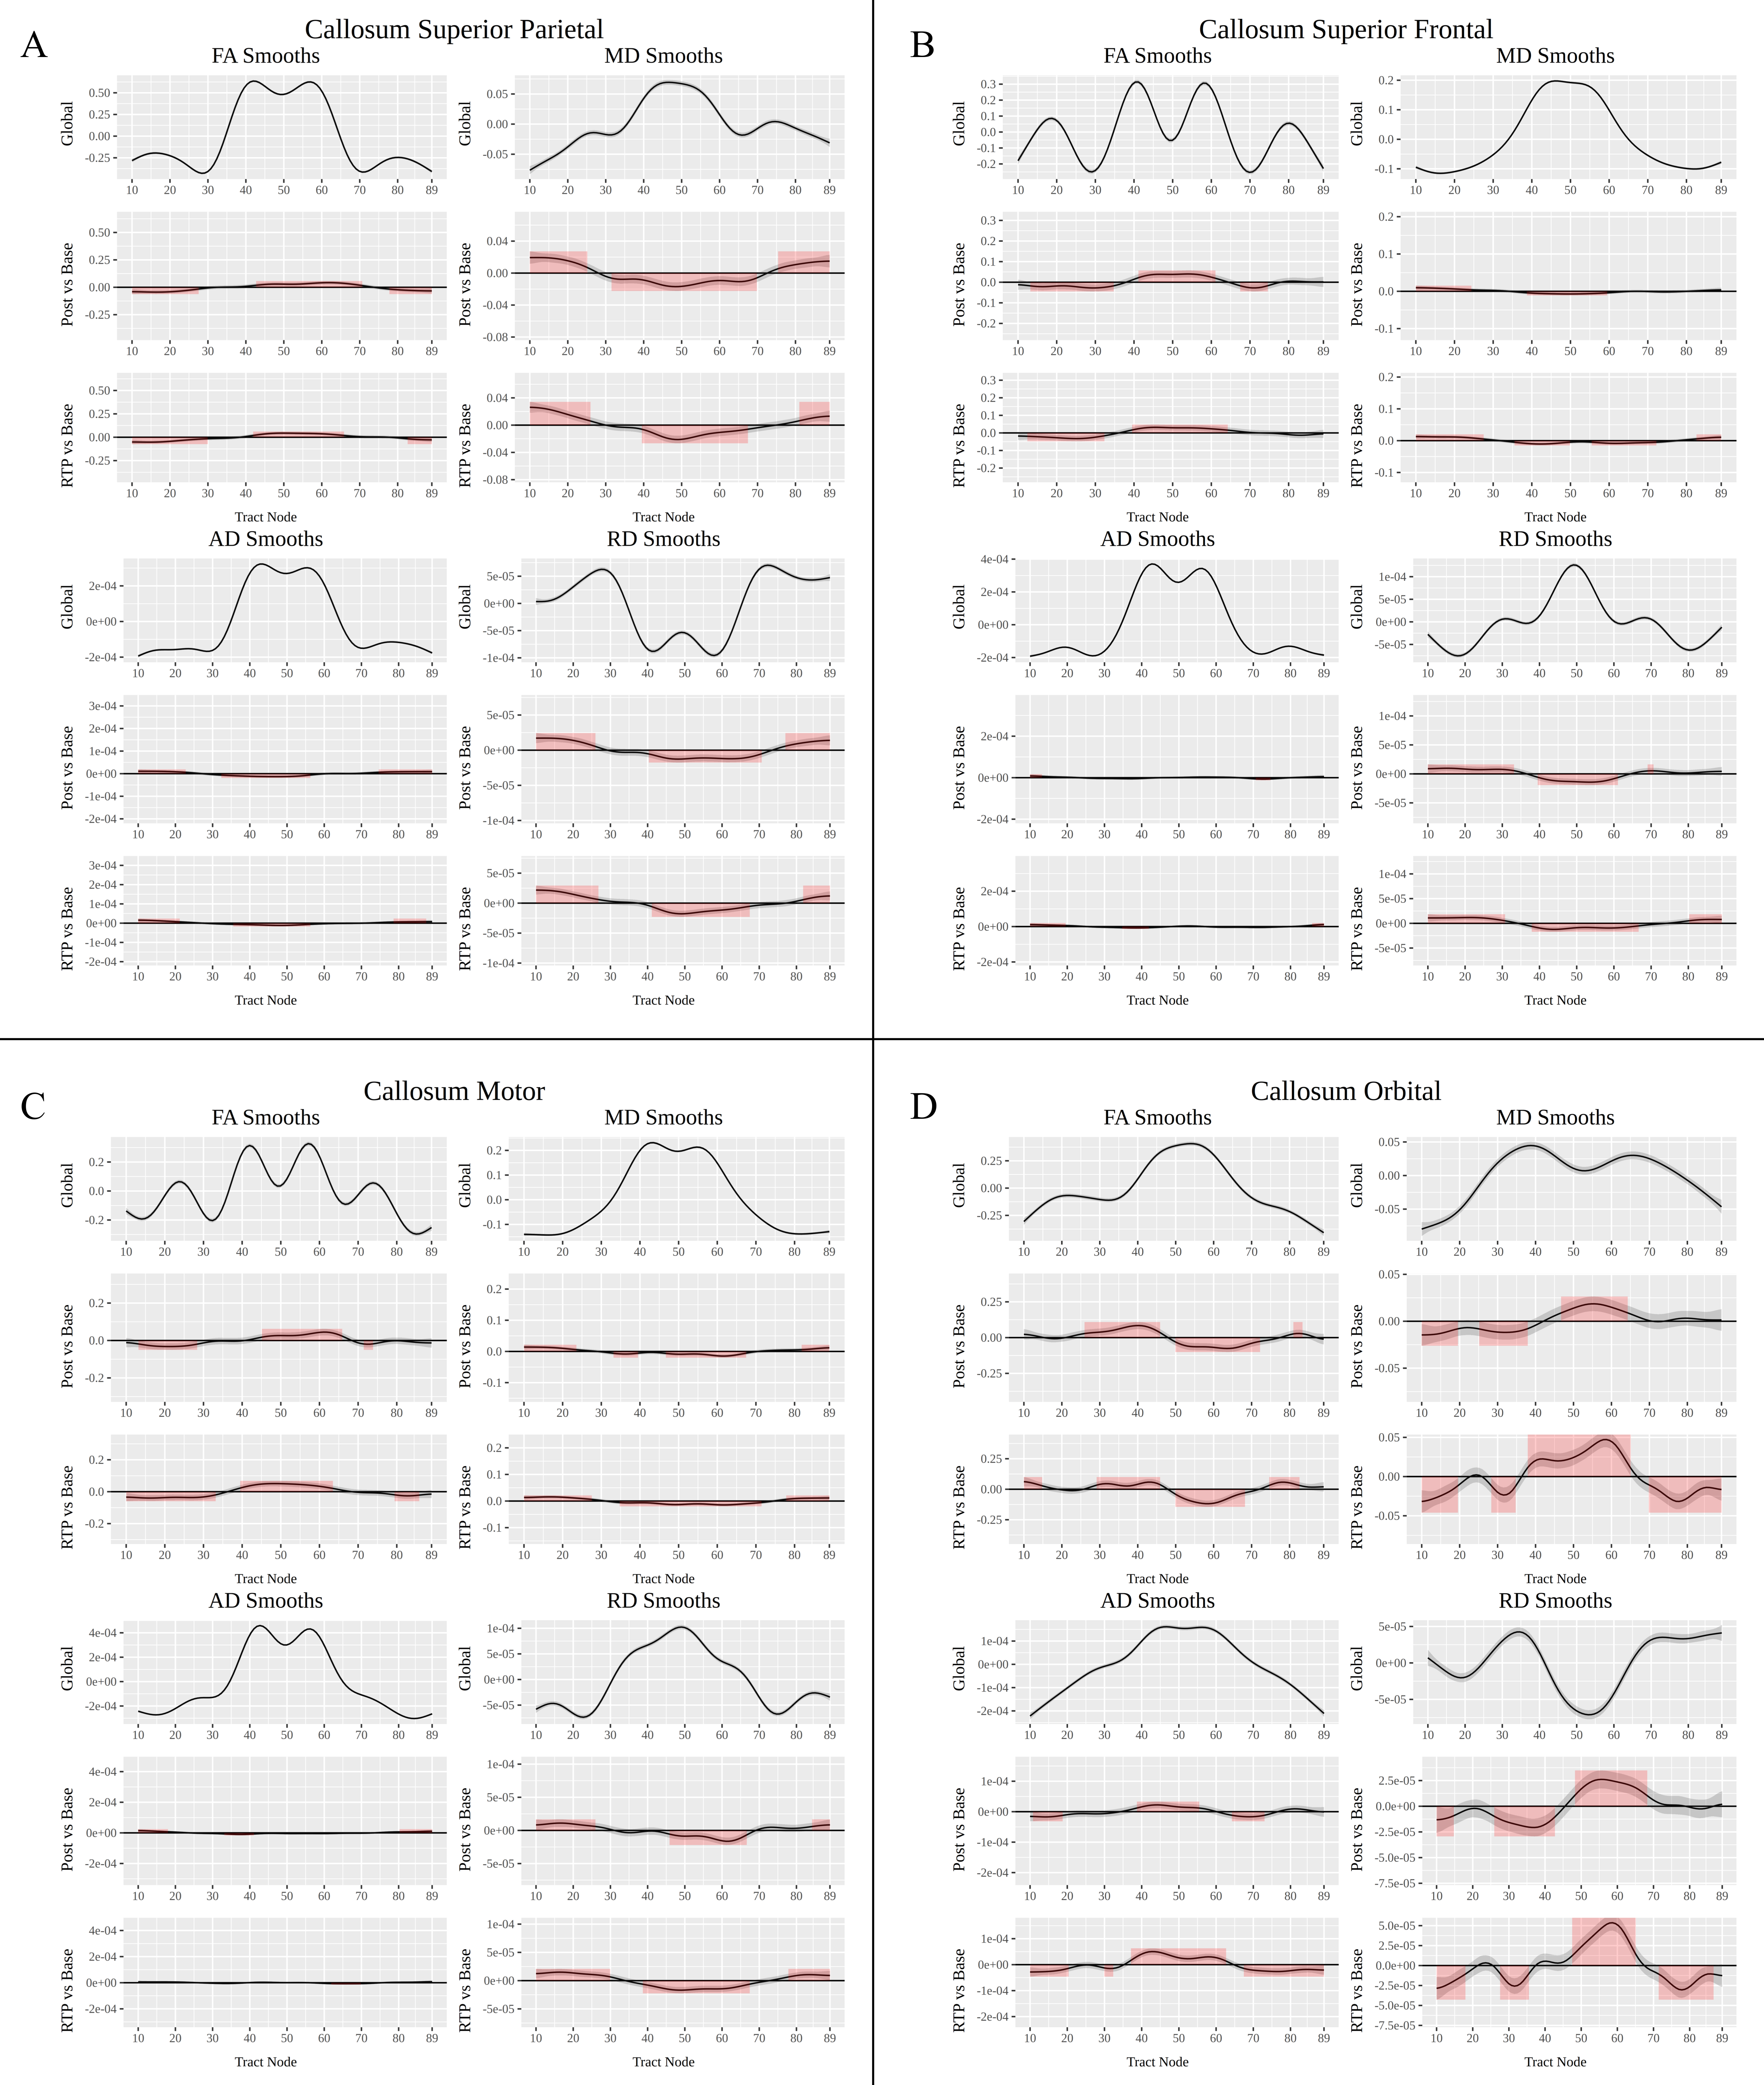
\includegraphics[scale=0.11]{fig_LGIO_callosal_smooths.png}}
	\caption{Longitudinal HGAM smooths modeling callosal tract scalars as a function of node. Each model fit both the global tractometric profile (global smooths) and how sessions differed from the global (group smooths). Group smooths (\lstinline{Diff: Post-Base}, \lstinline{Diff: RTP-Base}) are `difference from Base' smooths. \textbf{A}: Global and group smooths for Callosum Superior Parietal for FA (top left), MD (top right), AD (bottom left), and RD (bottom right). \textbf{B}: Global and group scalar smooths for Callosum Superior Frontal. \textbf{C}: Global and group scalar smooths for Callosum Motor. \textbf{D}: Global and group scalar smooths for Callosum Orbital. Red boxes indicate nodes where smooths differ statistically from the reference group (Base). Group smooths are plotted in the domain of the global smooth to show their fit contribution. LGIO = Longitudinal HGAM with Global and group (I) smooths, and an Ordered group factor.}
	\label{fig:lgio-gam-cc}
\end{figure}

These patterns of concussion- and recovery-related scalar changes partially confirms our second hypothesis that FA decreases would be driven by increased RD. While the expected directionality of injury-related scalar changes was only detected in the orbital tract (Figure \ref{fig:lgio-gam-cc}, D), we nevertheless observed that changes in FA were largely driven by RD and not AD.


\textit{Select Tract Results}. In addition to those of the corpus callosum, we identified a subset of tracts that showed concussion- and/or recovery-related scalar changes with magnitudes larger than were expected from algorithmic variance: left arcuate, left corticospinal, right anterior thalamic, right cingulum cingulate, right inferior fronto-occipital, and right uncinate (Figure \ref{fig:lgio-gam-sel}). Test statistics (Table \ref{tbl:lgio-gam-cc}) indicated that all ordered group smooths differed significantly from Base in at least one region of nodes, save for the left arcuate Post FA and left corticospinal Post AD smooths (Figure \ref{fig:lgio-gam-sel}, A \& B).

\begin{figure}[H]
	\centering
	\fbox{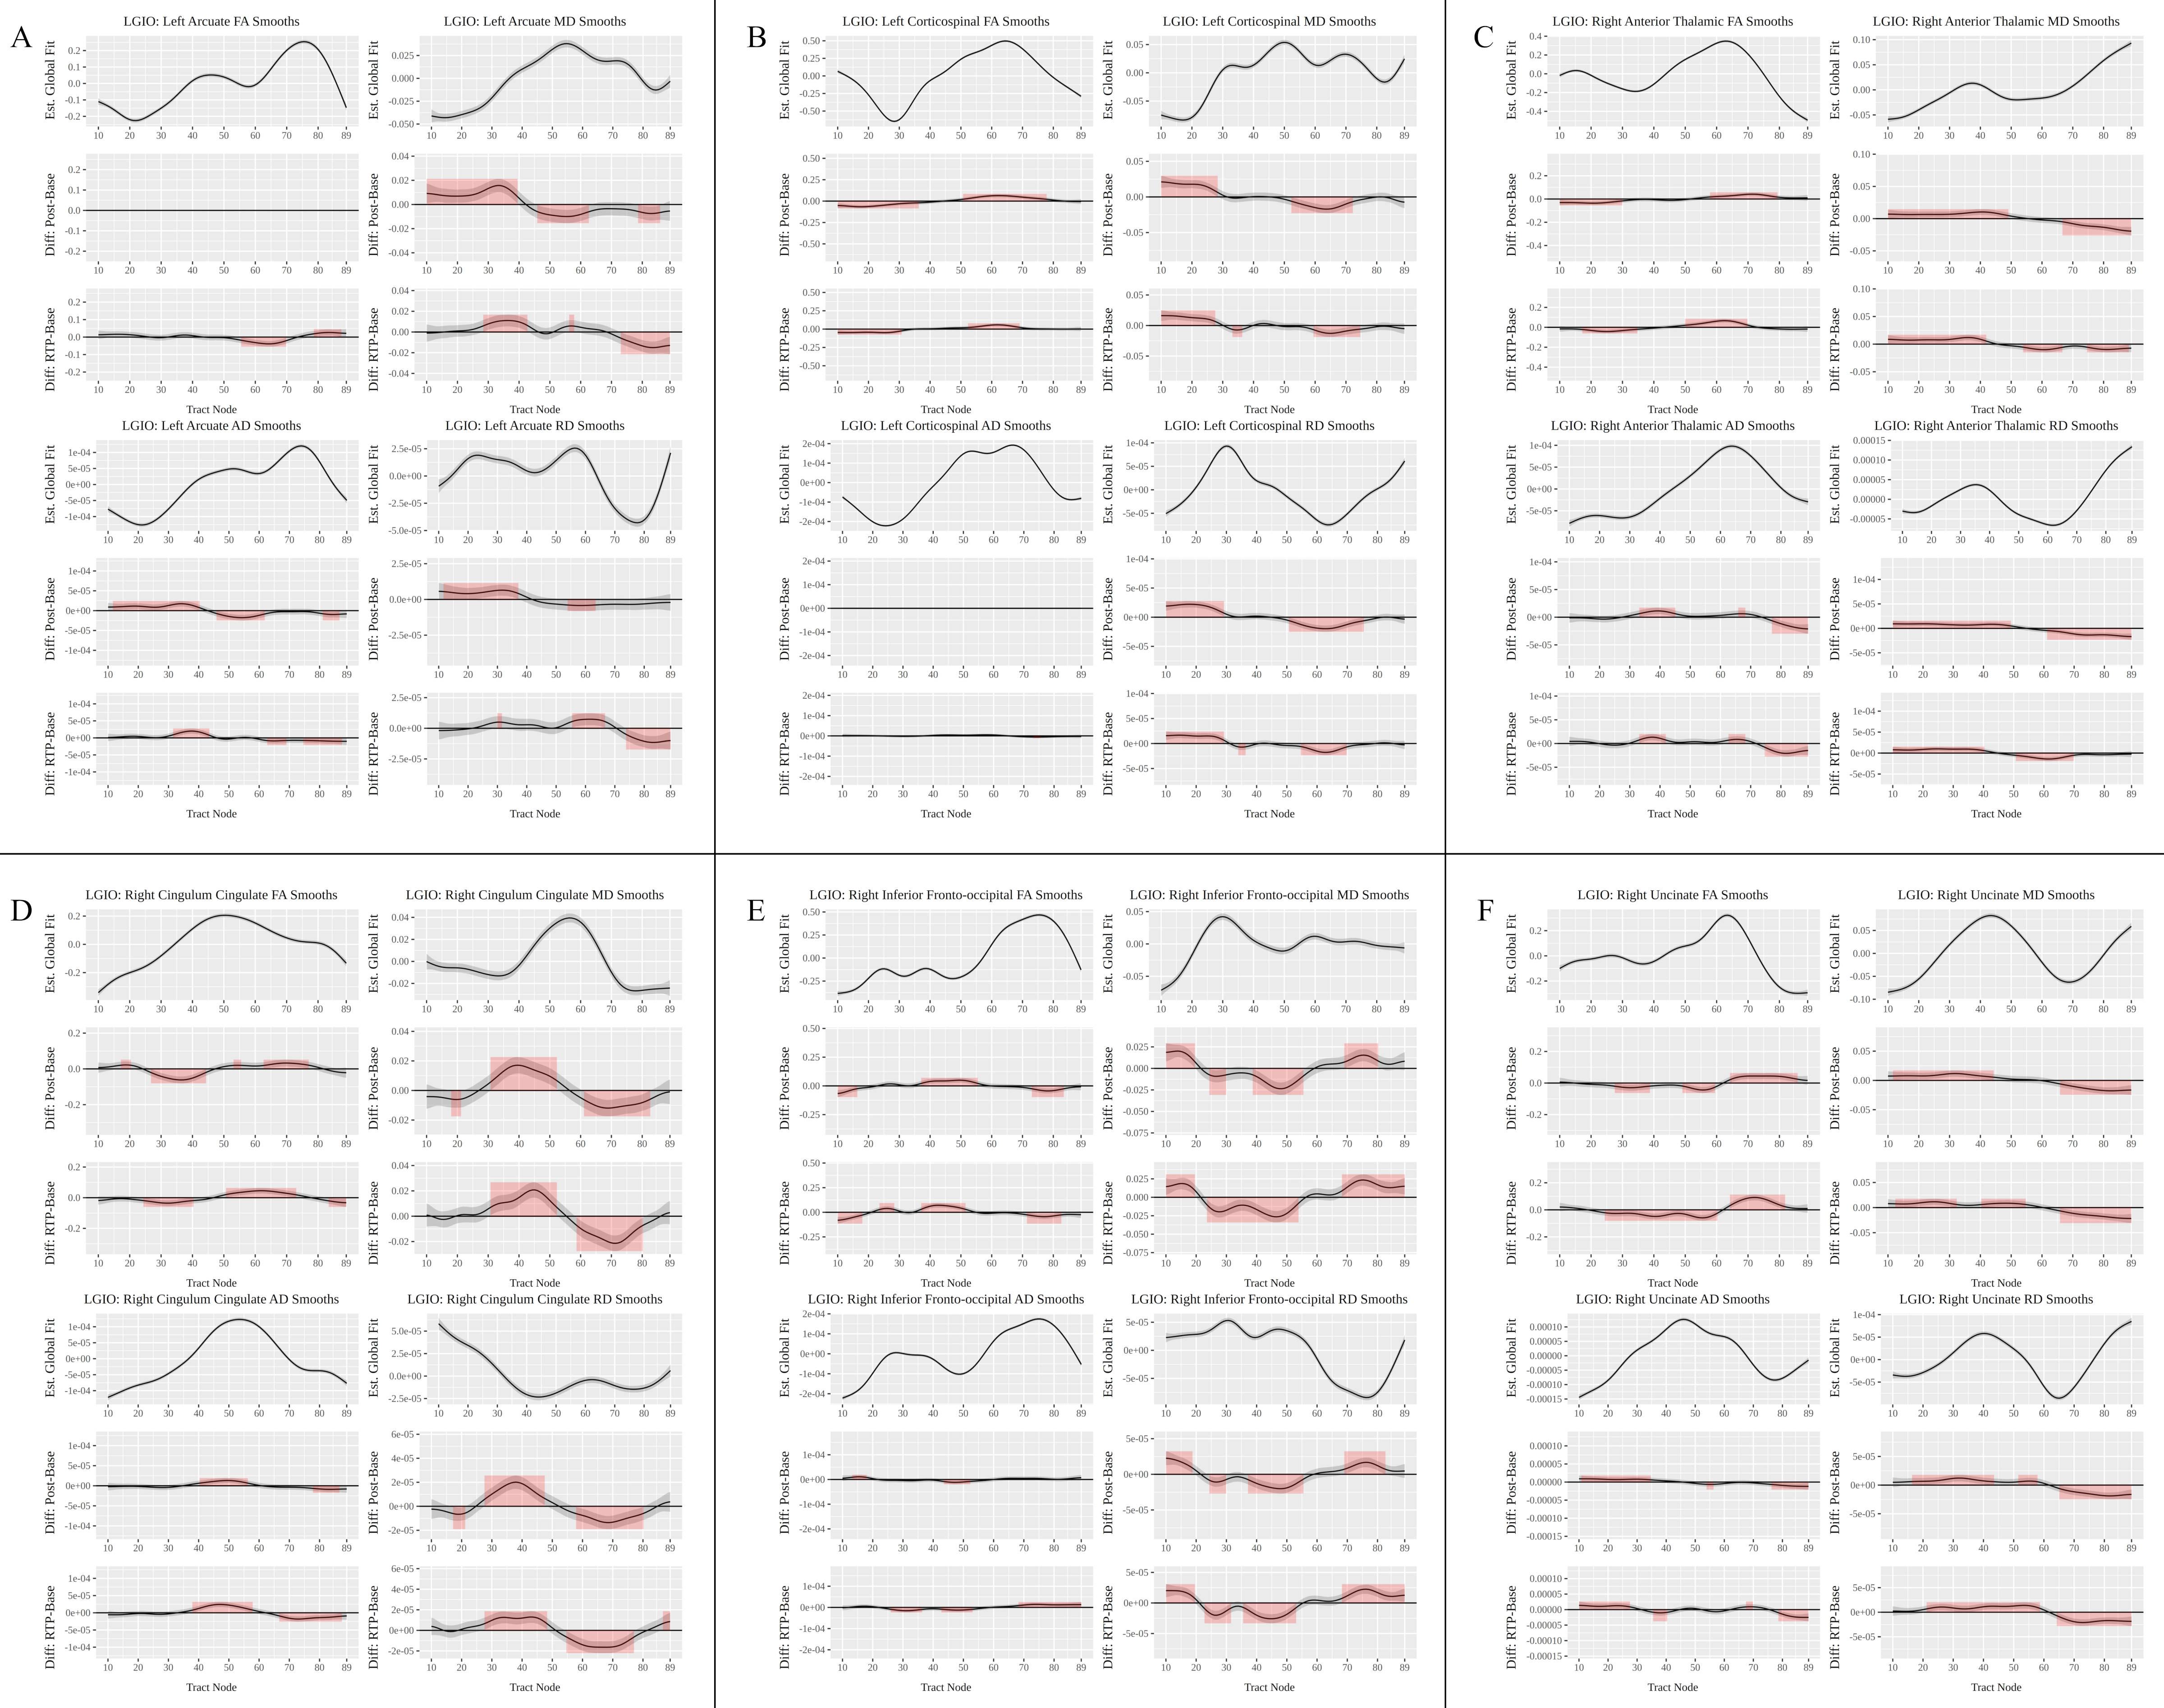
\includegraphics[scale=0.09]{fig_LGIO_select_smooths.png}}
	\caption{Longitudinal HGAM smooths modeling select tract scalars as a function of node. Each section (A-F) consists of global and session smooths for FA (top left), MD (top right), AD (bottom left), and RD (bottom right). Red boxes indicate nodes where smooths differ statistically from the reference group (Base). Group smooths are plotted in the domain of the global smooth to show their fit contribution. LGIO = Longitudinal HGAM with Global and group (I) smooths, and an Ordered group factor.}
	\label{fig:lgio-gam-sel}
\end{figure}

Within these selected tracts, and as with the callosal tracts, patterns of injury stability, recovery, and worsening are present. First, the corticospinal, anterior thalamic, and inferior fronto-occipital appear to have stable FA changes relative to Base. For the corticospinal, increases in FA (Figure \ref{fig:lgio-gam-sel}B, node 65) are driven by decreases in RD for the same region, and this pattern is also found for rIFO (Figure \ref{fig:lgio-gam-sel}E, node 45). For anterior thalamic, both decreases in RD and increases in AD are associated with the increase in FA values (Figure \ref{fig:lgio-gam-sel}C, node 65). Second, the arcuate and uncinate tracts both show evidence of worsening, where tract scalar become more discrepant with Base by RTP. At Post, the arcuate FA values do not differ from Base (albeit the increases in MD, AD, and RD; Figure \ref{fig:lgio-gam-sel}A), and by RTP a steep decrease in FA about node 65 is present which is driven by corresponding increase in RD. Likewise, the FA values for uncinate worsen over time (Figure \ref{fig:lgio-gam-sel}F), most dramatically in the increased FA values near node 70, an increase which is driven by RD decreases. Finally, the cingulum cingulate (Figure \ref{fig:lgio-gam-sel}D) shows evidence of recovery near node 35. At Post, a steep decrease in FA is associated with a corresponding increase in RD, which diminishes by RTP. That said, the slight increase in FA about node 70 at Post seems to elongate by RTP, with a decline in RD as well.

Together, these results largely mirror those detected in the callosal tracts. FA increases driven by RD decreases are commonly implicated in cytotoxic edema, while the reverse can be understood in terms of axolemmal permeability. Similarly, a number of tracts were detected to seemingly recover to Base values by RTP, with a few problematic tracts showing late emergent pathology.


\subsection{Tract FA Differences Relate to Changes in ImPACT Scores}
\label{ssec:res-dwi-imp}
\textit{Corpus Callosum Interaction Results}. Tensor product interaction smooths support multimodal interaction models. In addition to modeling within-tract longitudinal scalar changes, clinical assessment metrics (or data from other modalities) can be included in higher dimensional models (R Code \ref{code:gam-lgio-intx}) to investigate whether such assessment metrics relate to within-tract concussion-related scalar changes. We conducted exploratory analyses to determine whether changes in callosal FA values related to ImPACT composite and total symptom scores. Specifically, we tested whether the tract FA-ImPACT interaction at Post and RTP differed from those at Base, where Post differences may link physiologic changes (tract scalars) to clinical assessment and a lack of such differences at RTP may indicate recovery.

Of the eight callosal tracts tested, only three demonstrated the hypothesized interaction (Figure \ref{fig:intro-hyp}, right), where estimated FA values would relate to ImPACT scores within a discrete region of the tract at Post but not RTP. Specifically, the superior frontal FA changes interacted with changes in both visual memory and total symptom scores, occipital FA changes interacted with visual motor, and superior parietal with total symptom scores. Test statistics (Table \ref{tbl:lgio-intx-cc}, top) indicate that while controlling for the curvature of the tract (Global) and the main interaction effect (ImPACT-Node), a significant differential interaction exists at Post relative to Base (ImPACT-Node:O.Post) that is also reduced at RTP (ImPACT-Node:O.RTP).

\begin{table}[H]
	\scriptsize
	% Please add the following required packages to your document preamble:
% \usepackage[table,xcdraw]{xcolor}
% Beamer presentation requires \usepackage{colortbl} instead of \usepackage[table,xcdraw]{xcolor}

\begin{tabular}{lllllllllllll}
 & \multicolumn{3}{c|}{CCsf: VisMem} & \multicolumn{3}{c|}{CCsf: TotSymp} & \multicolumn{3}{c|}{CCocc: VisMot} & \multicolumn{3}{c}{CCsp: TotSymp} \\ \cline{2-13}
Smooth & \multicolumn{1}{c}{edf} & \multicolumn{1}{c}{F} & \multicolumn{1}{c|}{Sig} & \multicolumn{1}{c}{edf} & \multicolumn{1}{c}{F} & \multicolumn{1}{c|}{Sig} & \multicolumn{1}{c}{edf} & \multicolumn{1}{c}{F} & \multicolumn{1}{c|}{Sig} & \multicolumn{1}{c}{edf} & \multicolumn{1}{c}{F} & \multicolumn{1}{c}{Sig} \\ \hline
\multicolumn{1}{l|}{Node} & 13.95 & 775.40 & \multicolumn{1}{l|}{***} & 13.93 & 527.98 & \multicolumn{1}{l|}{***} & 13.79 & 2681.43 & \multicolumn{1}{l|}{***} & 13.92 & 2378.29 & *** \\
\rowcolor[HTML]{C0C0C0}
\multicolumn{1}{l|}{\cellcolor[HTML]{C0C0C0}ImP:Base} & 1.00 & 0.92 & \multicolumn{1}{l|}{\cellcolor[HTML]{C0C0C0}} & 1.00 & 1.25 & \multicolumn{1}{l|}{\cellcolor[HTML]{C0C0C0}} & 1.76 & 1.12 & \multicolumn{1}{l|}{\cellcolor[HTML]{C0C0C0}} & 1.69 & 0.77 &  \\
\multicolumn{1}{l|}{ImP:Post} & 1.00 & 3.64 & \multicolumn{1}{l|}{} & 1.00 & 3.08 & \multicolumn{1}{l|}{} & 1.01 & 0.01 & \multicolumn{1}{l|}{} & 2.77 & 1.87 &  \\
\rowcolor[HTML]{C0C0C0}
\multicolumn{1}{l|}{\cellcolor[HTML]{C0C0C0}ImP:RTP} & 1.00 & 0.17 & \multicolumn{1}{l|}{\cellcolor[HTML]{C0C0C0}} & 1.34 & 0.25 & \multicolumn{1}{l|}{\cellcolor[HTML]{C0C0C0}} & 1.01 & 0.21 & \multicolumn{1}{l|}{\cellcolor[HTML]{C0C0C0}} & 1.35 & 0.31 &  \\
\multicolumn{1}{l|}{ImP-Node} & 37.14 & 1.93 & \multicolumn{1}{l|}{***} & 37.56 & 2.83 & \multicolumn{1}{l|}{***} & 61.19 & 7.50 & \multicolumn{1}{l|}{***} & 46.82 & 3.72 & *** \\
\rowcolor[HTML]{C0C0C0}
\multicolumn{1}{l|}{\cellcolor[HTML]{C0C0C0}ImP-Node:O.Post} & 51.17 & 7.09 & \multicolumn{1}{l|}{\cellcolor[HTML]{C0C0C0}***} & 46.69 & 5.67 & \multicolumn{1}{l|}{\cellcolor[HTML]{C0C0C0}***} & 53.13 & 5.68 & \multicolumn{1}{l|}{\cellcolor[HTML]{C0C0C0}***} & 53.46 & 3.99 & *** \\
\multicolumn{1}{l|}{ImP-Node:O.RTP} & 36.16 & 1.83 & \multicolumn{1}{l|}{***} & 22.24 & 1.25 & \multicolumn{1}{l|}{***} & 39.66 & 1.72 & \multicolumn{1}{l|}{***} & 20.16 & 1.12 & *** \\ \hline
 &  &  &  &  &  &  &  &  &  &  &  &  \\
 & \multicolumn{3}{c|}{lCS} & \multicolumn{3}{c|}{rUnc} & \multicolumn{3}{c|}{CCocc} & \multicolumn{3}{c}{CCsp} \\ \cline{2-13}
Smooth & \multicolumn{1}{c}{edf} & \multicolumn{1}{c}{F} & \multicolumn{1}{c|}{Sig} & \multicolumn{1}{c}{edf} & \multicolumn{1}{c}{F} & \multicolumn{1}{c|}{Sig} & \multicolumn{1}{c}{edf} & \multicolumn{1}{c}{F} & \multicolumn{1}{c|}{Sig} & \multicolumn{1}{c}{edf} & \multicolumn{1}{c}{F} & \multicolumn{1}{c}{Sig} \\ \hline
\multicolumn{1}{l|}{Node} & 5.77 & 4.06 & \multicolumn{1}{l|}{***} & 1.80 & 0.47 & \multicolumn{1}{l|}{} & 4.88 & 4.95 & \multicolumn{1}{l|}{***} & 3.90 & 3.45 & ** \\
\rowcolor[HTML]{C0C0C0}
\multicolumn{1}{l|}{\cellcolor[HTML]{C0C0C0}Days} & 1.00 & 3.68 & \multicolumn{1}{l|}{\cellcolor[HTML]{C0C0C0}} & 1.08 & 1.52 & \multicolumn{1}{l|}{\cellcolor[HTML]{C0C0C0}} & 1.19 & 0.72 & \multicolumn{1}{l|}{\cellcolor[HTML]{C0C0C0}} & 1.00 & 0.42 &  \\
\multicolumn{1}{l|}{Days-Node} & 37.10 & 2.04 & \multicolumn{1}{l|}{***} & 38.39 & 2.25 & \multicolumn{1}{l|}{***} & 35.40 & 1.60 & \multicolumn{1}{l|}{***} & 32.55 & 1.15 & ***
\end{tabular}

	\caption{Longitudinal tract interaction statistics. \textbf{Top}: Interaction of callosal tracts and ImPACT metrics. While significant non-flatness is detected for all ImPACT-Node interactions, note the reduction in effective degrees of freedom and F-stat between Post and RTP. VisMem = Visual Memory, TotSymp = Total Symptom, VisMot = Visual Motor. Node = global node, ImP:Base/Post/RTP = main effects of ImPACT metric for each group, ImP-Node = interaction term of node and ImPACT, ImP-Node:O.Post/RTP = Post/RTP group interaction as an ordered factor (relative to Base). \textbf{Bottom}: Interaction of select tracts and days between Post and RTP. edf = effective degrees of freedom, F = F-statistic, Sig = significance. *** = p$<$.001, ** = p$<$.01, * = p$<$.05.}
	\label{tbl:lgio-intx-cc}
\end{table}

Figure \ref{fig:lgio-intx-cc} visualizes Post and RTP tract node-FA-ImPACT difference interactions as topological surfaces to facilitate reviewing the pattern and magnitude of the tensor product interaction effects. A somewhat linear differential interaction at Post is found for each tract, and this difference from Base largely resolves by RTP. For instance, an interaction exists in the superior frontal tract about nodes 40-60 at Post (the same nodes which were implicated above) where lower visual memory scores are associated with decreased FA values (Figure \ref{fig:lgio-intx-cc}, A). At RTP, while a linear interaction is still somewhat present, the magnitude of the effect is diminished. Likewise, total symptoms are related to decreased FA values about superior frontal callosal nodes 40-60 (Figure \ref{fig:lgio-intx-cc}, B), poorer visual motor performance with nodes 40-50 of occipital (Figure \ref{fig:lgio-intx-cc}, C), and total symptoms with decreased FA superior parietal nodes 40-60 (Figure \ref{fig:lgio-intx-cc}, D). In each case of these cases, the FA-ImPACT interaction resolved by RTP, indicated by the `flatter' interaction difference surface (and fewer effective degrees of freedom and lower F-statistics in Table \ref{tbl:lgio-intx-cc}, top).

% TODO: Update interaction figures IMPACT -> ImPACT
% TODO: Update interaction figure titles Visit: Post-Base -> Post vs Base

\begin{figure}[H]
	\centering
	\fbox{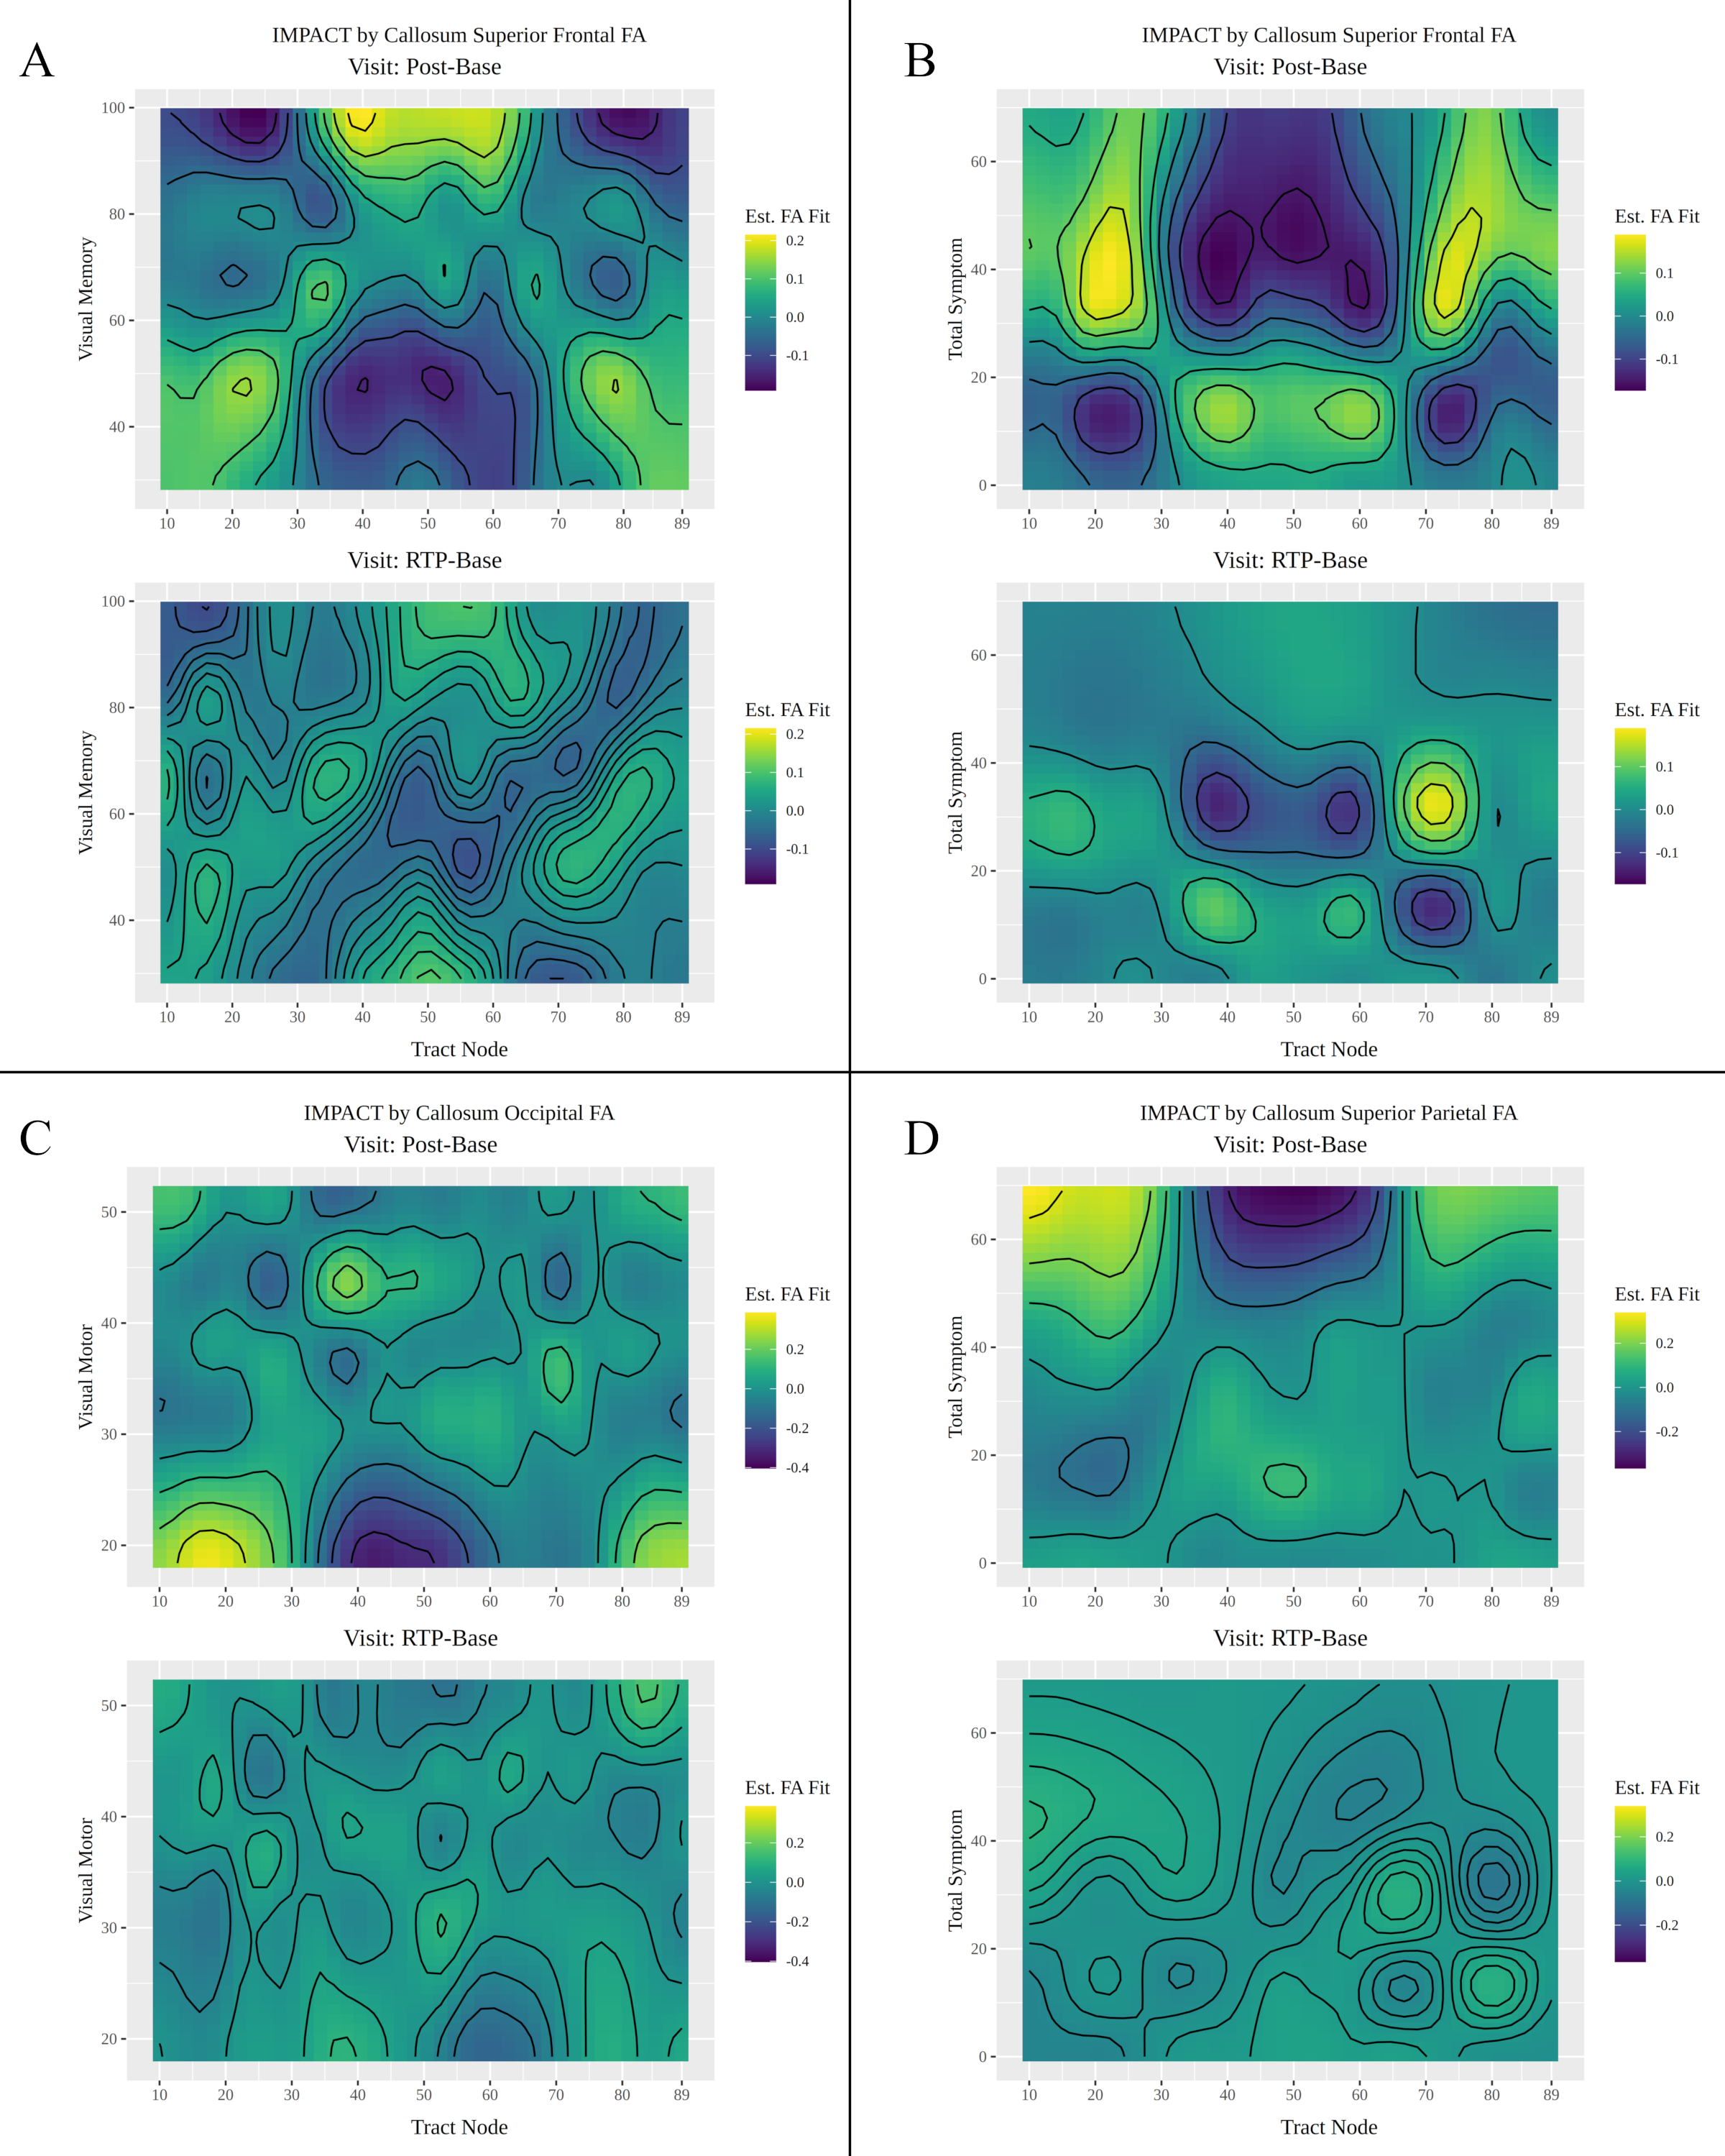
\includegraphics[width=0.9\textwidth]{fig_LGIO_intx_callosal.png}}
	\caption{HGAM tensor product interaction smooths testing for differences from Base node-FA-ImPACT interactions at Post and RTP. A linear interaction is present at Post in each quadrant (top plots), indicated by a gradient (Z) change along the Y-axis at a specific node (X) region. This interaction is diminished or not found at RTP (bottom plots).}
	\label{fig:lgio-intx-cc}
\end{figure}


% TODO: should select tract interaction results be kept?
\textit{Select Tract Interaction Results}. Further exploratory analyses were conducted to see whether scalar changes in selected tracts (Figure \ref{fig:lgio-gam-sel}) related to changes in ImPACT composite and total symptom scores. Surprisingly, of the tracts and ImPACT metrics tested, the hypothesized interaction was only detected between the left corticospinal tract and reaction time (Figure \ref{fig:lgio-intx-lcs}; Global $F_{(13.62, 13.94)}$ = 1695.79, \textit{p} $<$ .001; Impact:Base $F_{(1, 1)}$ = 0.2, \textit{p} $=$ .65; Impact:Post $F_{(1, 1)}$ = 0.05, \textit{p} $=$ .82; Impact:RTP $F_{(1, 1)}$ = 1.07, \textit{p} $=$ .29; Impact-Node $F_{(39.33, 76)}$ = 2.56, \textit{p} $<$ .001; Impact-Node:O.Post $F_{(44.17, 76)}$ = 2.29, \textit{p} $<$ .001; Impact-Node:O.RTP $F_{(44.36, 76)}$ = 1.64, \textit{p} $<$ .001). At Post, the slowest reaction times were associated with larger FA values about node 75. This pattern is reversed at RTP, likely due to sparsity in slow reaction times given recovery (see Figure \ref{fig:imp-gam}, bottom right).

\begin{figure}[H]
	\centering
	\fbox{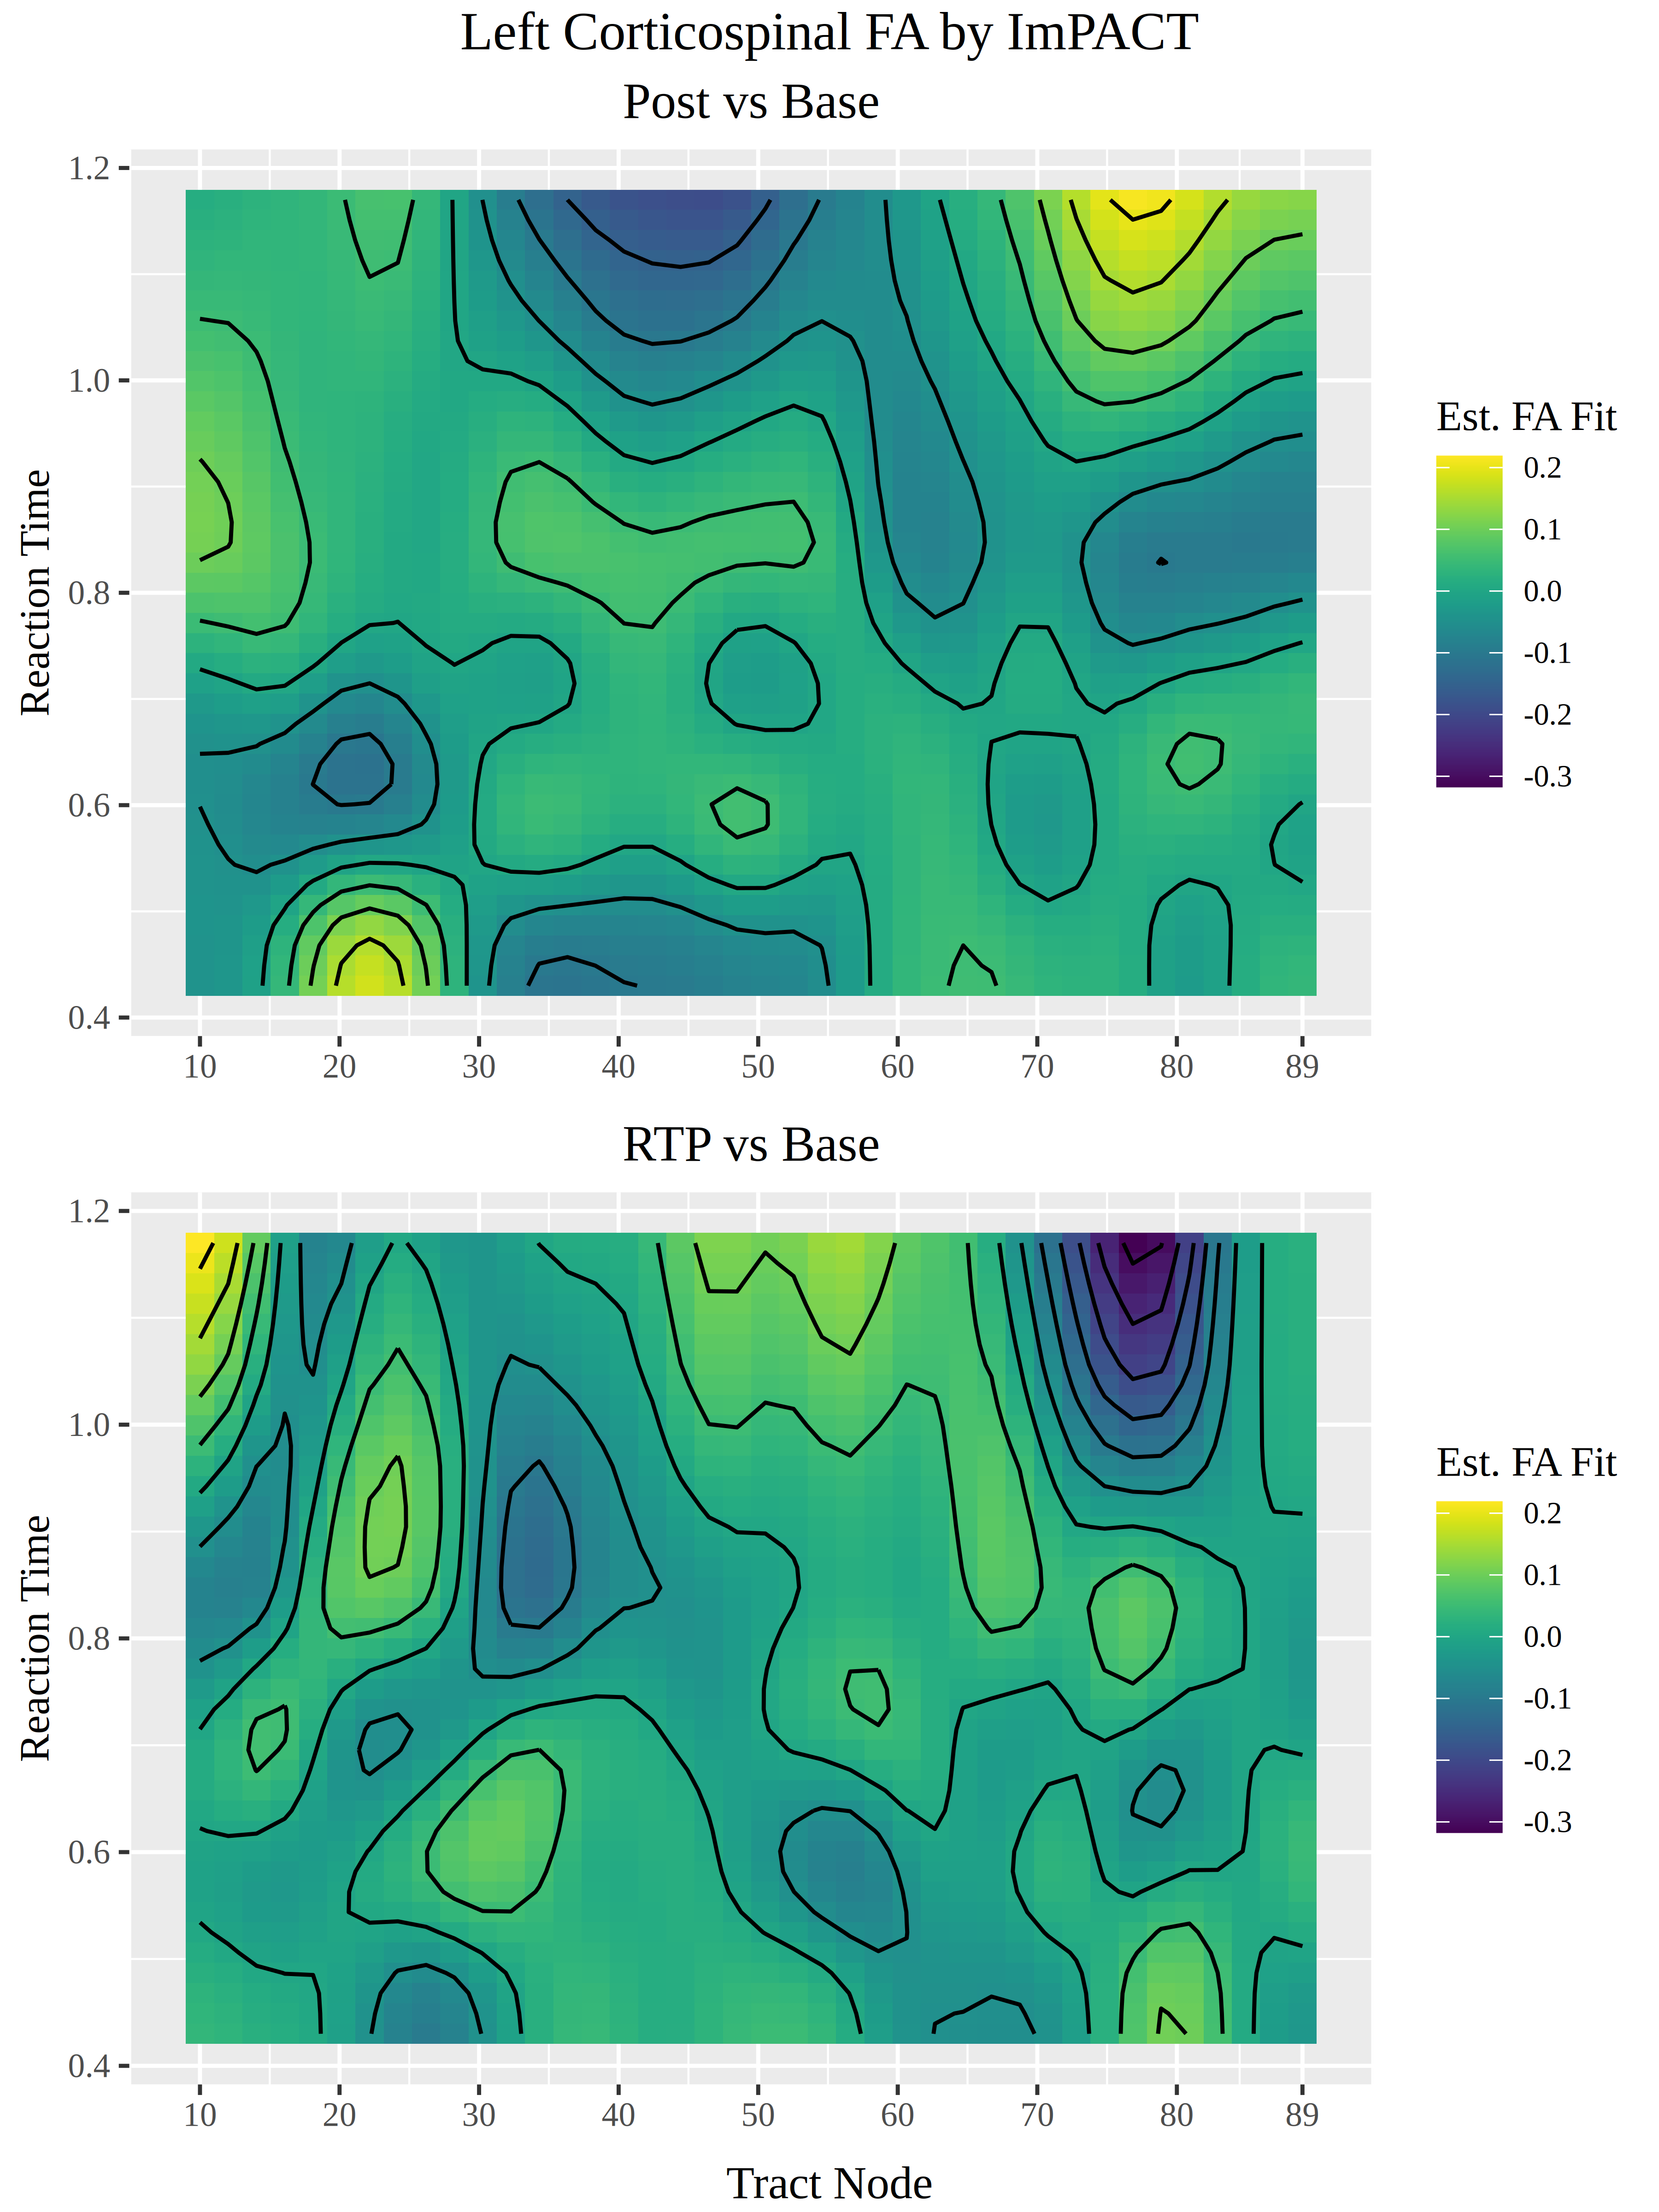
\includegraphics[width=0.5\textwidth]{fig_LGIO_intx_lCS_rx_time.png}}
	\caption{HGAM tensor product interaction of node, FA, and reaction time for the left Corticospinal tract. Post and RTP surfaces are relative to Base. Rx Time = reaction time.}
	\label{fig:lgio-intx-lcs}
\end{figure}


\subsection{Tract FA Difference Relate to Recovery Time}
\label{ssec:res-dwi-time}
In addition to modeling the interaction of tract FA changes with assessment metrics (Section \ref{ssec:res-dwi-imp}), another potentially powerful use of tensor product interaction smooths is to model changes in tract scalars as a function of time. Given the within-tract temporal dynamics of axonal injury and recovery, the ability to model non-linear temporal interactions with scalar changes will help quantify the progression of injury. For such an analysis, however, multiple scans would be required of each participant to effectively track signal associated with recovery. As our data were collected at Post and RTP, we modeled tract FA differences (for the tracts identified above) between Post and RTP as a function of node and number of days between the two sessions. Such a model will identify which scalar changes are associated with the longest recovery periods, as presumably less-severe injuries are associated with fewer days between Post and RTP. We also note that few participants had recovery periods longer than 14 days, so any detected interactions at long recovery periods are driven by relatively few participants.

Our hypothesized interaction was identified in two node-$\Delta$FA-time patterns which are visualized as topographic maps in Figure \ref{fig:di-time} (also, Table \ref{tbl:lgio-intx-cc}, bottom). First, positive $\Delta$FA values were associated with longer recovery periods in the left corticospinal (node 50) and right uncinate (node 55) tracts (Figure \ref{fig:di-time}, A \& B), and negative $\Delta$FA values in the left corticospinal tracts related to a shorter recovery period. A positive RTP-Post $\Delta$FA may indicate significant axolemmal damage at Post which would have decreased Post FA and preceded a longer recovery period, while a negative difference value might occur when slight edema is present at Post (increased FA, decreased RD, no change in AD) which then resolves by RTP. Second, negative RTP-Post $\Delta$FA values in the superior parietal (node 55) and orbital callosal (node 60) tracts were related to longer recovery periods (Figure \ref{fig:di-time}, C \& D). It is possible, as with the corticospinal tract, that such negative $\Delta$FA values could be driven by significant axonal swelling at Post, resulting in a decreased RD and therefore increased FA. Shorter recovery periods, however, did not have a clear relationship with $\Delta$FA values in these tracts, as indicated by the flat (homogeneous green) regions of the tensor product interaction smooths.


\begin{figure}[H]
	\centering
	\fbox{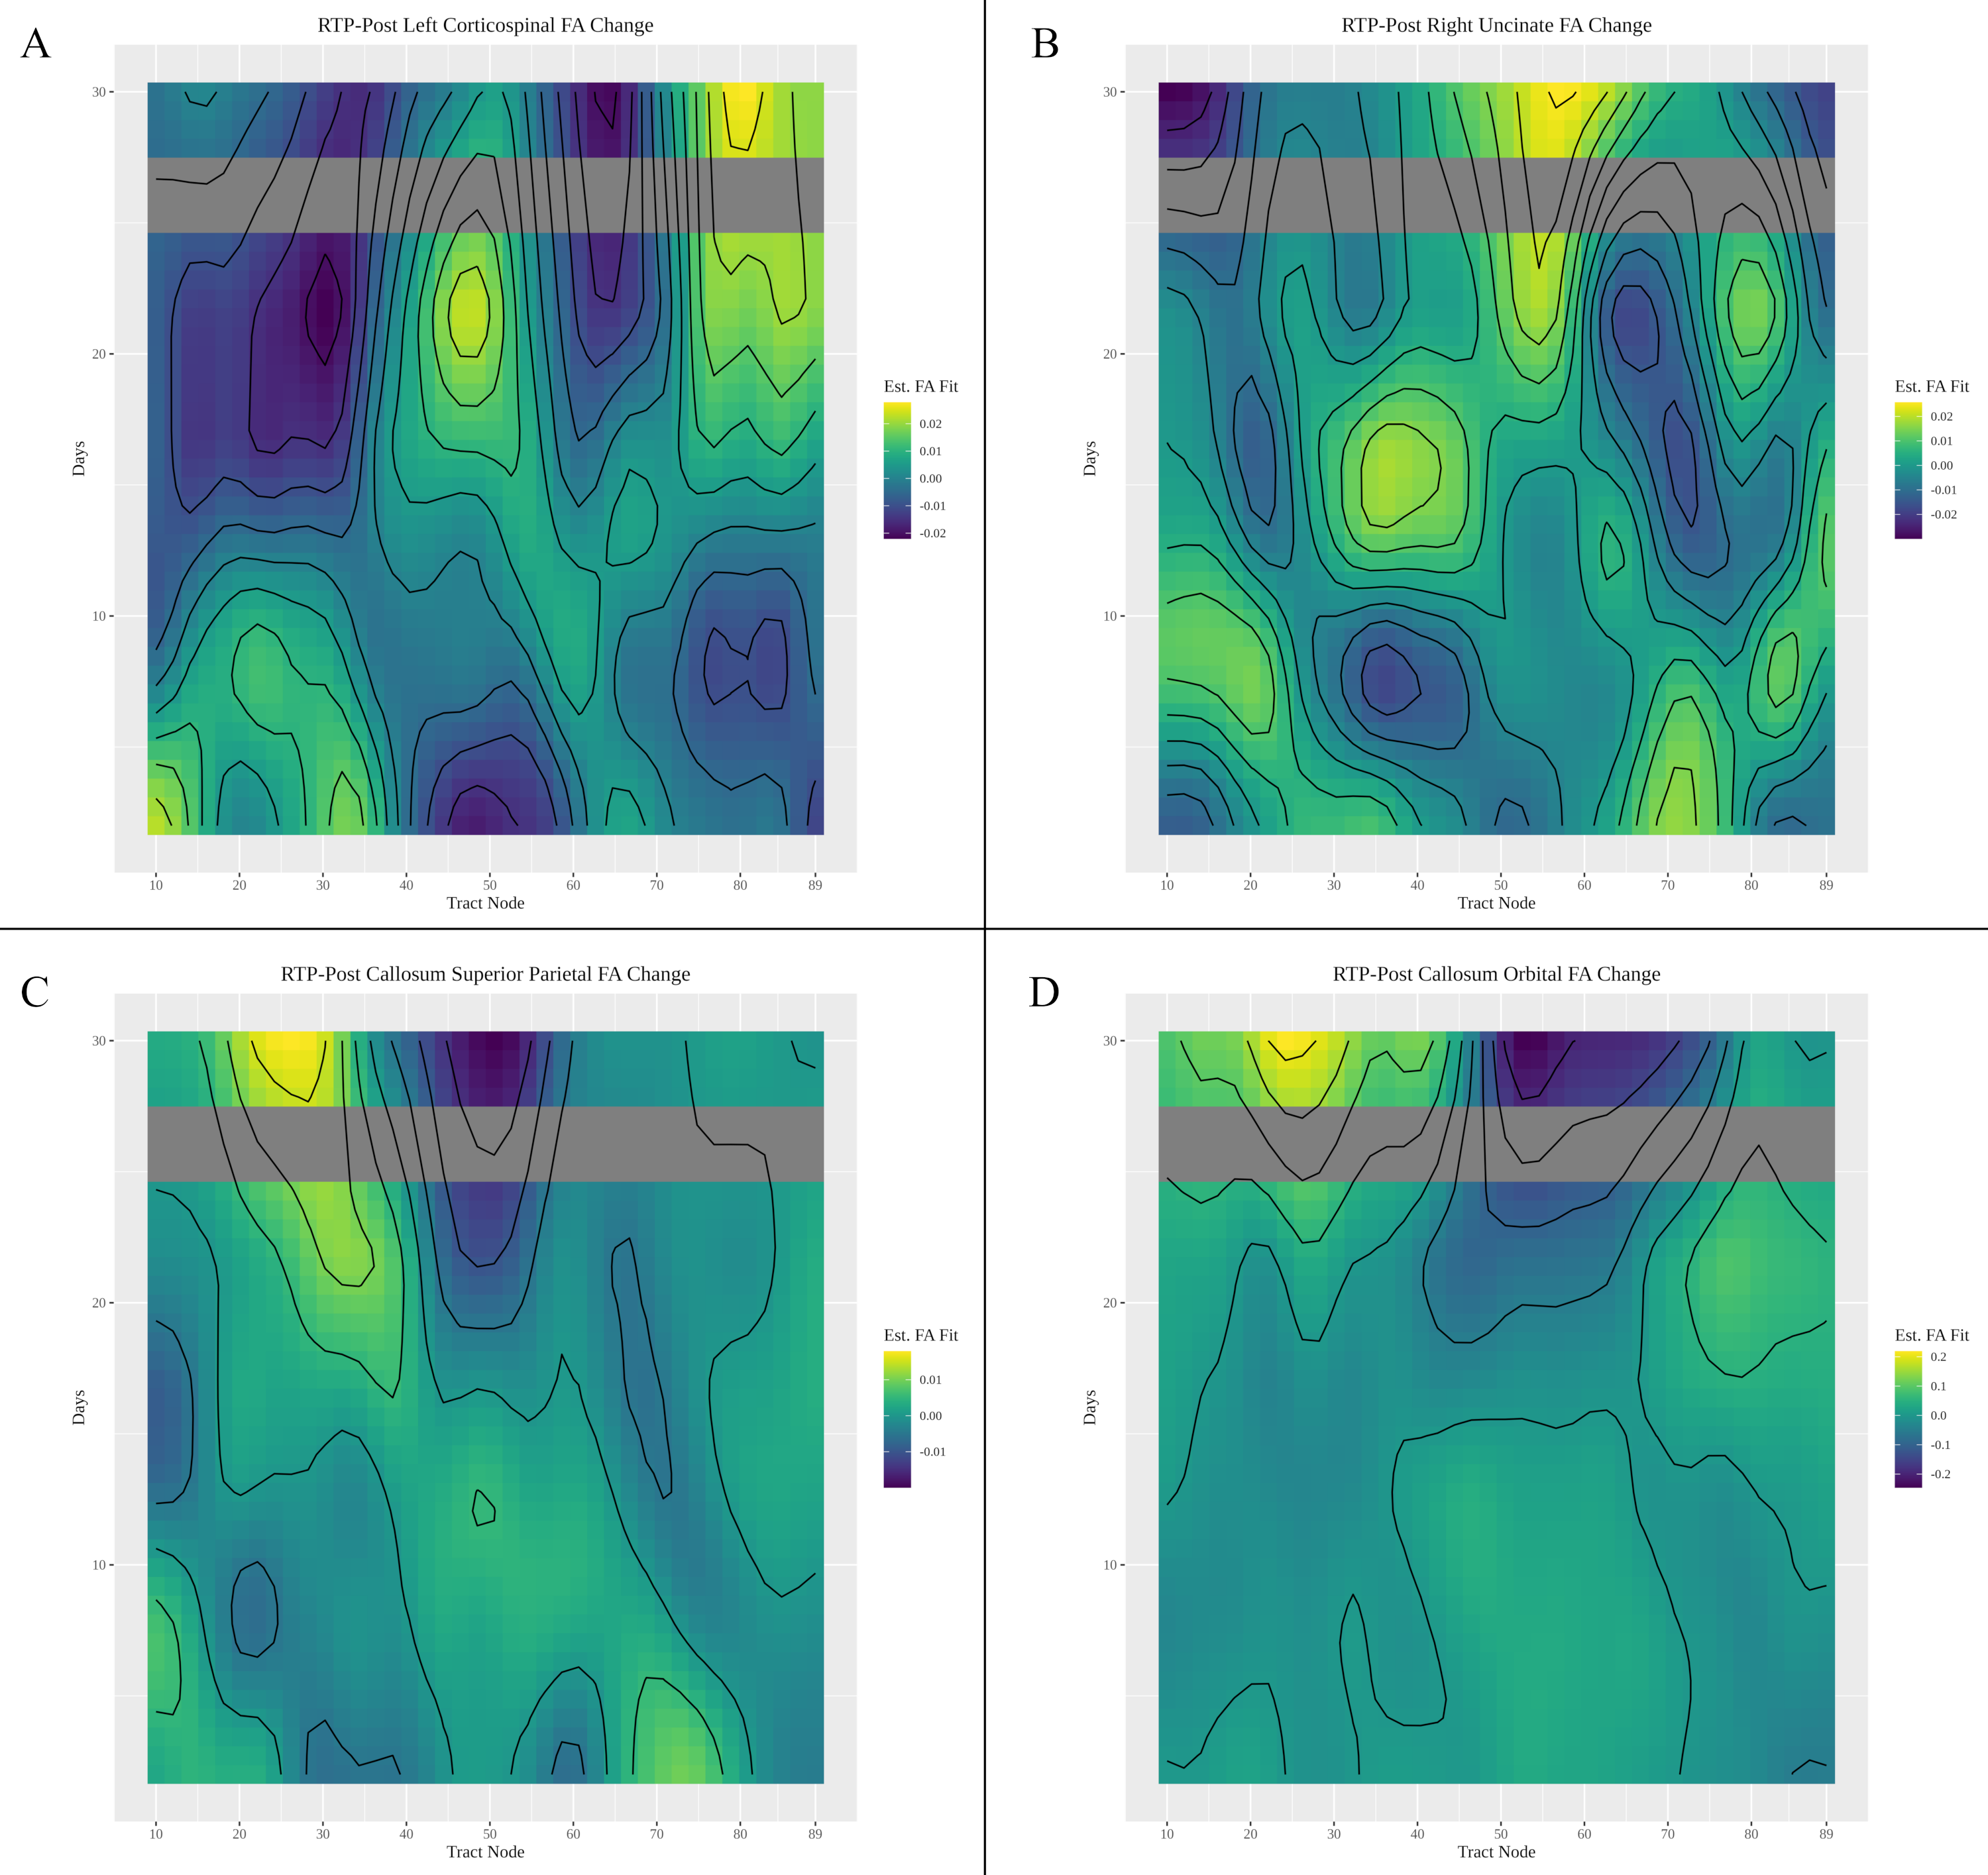
\includegraphics{fig_DI_time.png}}
	\caption{HGAM tensor product interaction smooths modeling the interaction between RTP-Post $\Delta$FA values (Z-axis) with the number of days between Post and RTP visits (Y-axis) along the tract nodes (X-axis). Positive RTP-Post $\Delta$FA values are indicated as yellow, and negative blue, with gray bars indicating regions of extrapolation (insufficient data). Top plots indicate positive $\Delta$FA values about node 50 are associated with a larger number of days between Post and RTP, and bottom plots the opposite.}
	\label{fig:di-time}
\end{figure}



\section{Discussion}
\label{sec:disc}
Discussion here.

% TODO: Summary/recap
% TODO: Interpret main findings
% TODO: Reversed smooth-tensor interactiosn -- different groups in data.
% TODO: Advocate HGAMs for mTBI research, reference AFQ-Insight?
% Limitations: Interpretation of statistic (flatness and LGI, LGIO models), all data in one model - underfit certain profiles, scan-rescan variance in addition to algorithmic, heterogeneity of injury and insufficient sample size to cluster symptom profiles, tensor products can be driven by sparesely sampling.


% acknowledgment page
\section*{Acknowledgments}
\label{sec:ack}
People. Grant.

% TODO: ariana for consulting


% write bibliography
\pagebreak
\printbibliography
\pagebreak


% make supplemental
\section{Supplemental Materials}
\label{sec:supp-materials}
\beginsupplement
Supplemental Materials.


\begin{equ}[H]
	\begin{lstlisting}
		fit_LGI <- mgcv::bam(
		  <scalar> ~ s(subj_id, scan_name, bs="re") +
		    s(node_id, bs="tp", k=15, m=2) +
		    s(node_id, by=scan_name, bs="tp", k=15, m=1),
		  data=df,
		  family=<family>,
		  method="fREML",
		  nthreads=4
		)
	\end{lstlisting}
	\caption{Tract scalars are modeled as a function of tract node with thin-plate regression splines using both global and group (\lstinline{scan_name}) smooths as well as individual group wiggliness. \lstinline{<scalar>} = relevant DWI metric (AD, RD, MD, or FA), \lstinline{scan_name} = session identifier factor (Base, Post, RTP), \lstinline{<family>} = relevant family and link function for scalar distribution.}
	\label{supp-code:gam-lgi}
\end{equ}


\begin{equ}[H]
	\begin{lstlisting}
		fit_LGI_intx <- mgcv::bam(
		  <scalar> ~ s(subj_id, scan_name, bs="re") +
		    s(node_id, bs="tp", k=15, m=2) +
		    s(imp_meas, by=scan_name, bs="tp", k=5) +
		    ti(
		      node_id, imp_meas, by=scan_name,
		      bs=c("tp","tp"), k=c(20,5), m=1
		    ),
		  data=df,
		  family=<family>,
		  method="fREML",
		  nthreads=4
		)
	\end{lstlisting}
	\caption{Tract scalars are modeled as a function of separate 1D node and ImPACT smooths as well as a 2D tensor product interaction surface. \lstinline{imp_meas} = ImPACT composite or total symptom measure.}
	\label{supp-code:gam-lgi-intx}
\end{equ}


\begin{equ}[H]
	\begin{lstlisting}
		fit_G <- mgcv::bam(
		  imp_meas ~ s(subj_id, bs="re") +
		    s(num_assess, bs="tp", k=3),
		  data=df,
		  family=<family>,
		  method="fREML"
		)
	\end{lstlisting}
	\caption{ImPACT metrics modeled as a function of number of assessments using a single global smooth. \lstinline{imp_meas} = ImPACT composite or total symptom score, \lstinline{num_assess} = assessment number (1=Base, 2=Post, 3=RTP).}
	\label{supp-code:gam-impact}
\end{equ}


\begin{equ}[H]
	\begin{lstlisting}
		fit_DI <- mgcv::bam(
		  delta_fa ~ s(subj_id, by=tract_name, bs="re") +
		    s(node_id, by=tract_name, bs="tp", k=15) +
		    tract_name,
		  data=df,
		  family=gaussian(),
		  method="fREML",
		  nthreads=12
		)
	\end{lstlisting}
	\caption{Run-Rerun $\Delta$FA values were modeled with node smooths for each tract.}
	\label{supp-code:gam-di}
\end{equ}

% \subsection{Tables}
% \label{ssec:supp-tables}
% Supplemental Tables.


% \subsection{Figures}
% \label{ssec:supp-figures}
% Supplemental Figures.


\end{document}